\documentclass{bmvc2k}
\usepackage{multicol}
\usepackage{minted}
\usepackage{float}

%% Enter your paper number here for the review copy
% \bmvcreviewcopy{??}

\title{dno}

% Enter the paper's authors in order
% \addauthor{Name}{email/homepage}{INSTITUTION_CODE}
\addauthor{Maciej A. Czyzewski}{inf136698}{1}

% Enter the institutions
% \addinstitution{Name\\Address}
\addinstitution{
	Poznan University of Technology \\
	Poland
}

\runninghead{Raport}{Informatyka w Medycynie}

% Any macro definitions you would like to include
% These are not defined in the style file, because they don't begin
% with \bmva, so they might conflict with the user's own macros.
% The \bmvaOneDot macro adds a full stop unless there is one in the
% text already.
\def\eg{\emph{e.g}\bmvaOneDot}
\def\Eg{\emph{E.g}\bmvaOneDot}
\def\etal{\emph{et al}\bmvaOneDot}

%-------------------------------------------------------------------------
% Document starts here
\begin{document}

\maketitle

%-------------------------------------------------------------------------

\section{Zastosowany język programowania oraz dodatkowe biblioteki}

Python. Lista bibliotek (niektore sluza tylko do debugowania):

\begin{multicols}{3}
\begin{itemize}
\item torchvision==0.4.2
\item scipy==1.3.1
\item numpy==1.17.2
\item matplotlib==3.1.1
\item torchsummary==1.5.1
\item torch==1.3.1
\item tqdm==4.36.1
\item scikit\_image==0.15.0
\item ipython==7.13.0
\item Pillow==7.1.0
\item scikit\_learn==0.22.2
\end{itemize}
\end{multicols}

\section{Opis zastosowanych metod}

Uczenie masznowe. Batchboost. Kfold. Augmentacja. Lamb Optimizer. Unet (wlasna
wersja ~400tys parametrow + batchnorm w bottlenecku). Taktyka tym razem jest
prosta. Pokroj obrazek na male kwadraciki (32x32px, albo podobne warianty).
Naucz sie rozpoznawac maske dla takiego malego obrazka. Nie przejmujemy sie
skutecznoscia jak wynosi juz okolo 80\%. Losujemy bardzo duzo malych wycinkow i usredniamy predykcje. Dzieki temu powinno
to jakos wygladac. Aby dzialaly wieksze wejscia niz 32x32 polecam zwiekszyc ilosc
warst sieci. Kfold-y pomogaja przy overfittingu (bardziej zdiagnozowac
raka niz go wyleczyc). Dlatego zastosowalem technike batchboost - efektem
jest
trening ktory zawsze ma wyzszy loss niz walidacja, oraz process stablizuje sie bedac bardziej
niezaleznym od parametrow.

\subsection{Przetwarzanie obrazów}

\subsubsection{Poszczególne kroki przetwarzania obrazu (w tym zastosowane filtrów)}

Kod jest bardzo czytelny - {\tt colab.py}. Ponizej najwazniesze wycinki.
\textbf{Preprocessing}:

\begin{minted}[mathescape,
               linenos,
               numbersep=5pt,
               gobble=0,
               frame=lines,
			   framesep=2mm]{python}
@staticmethod
def block(img):
	# FIXME: grid searchowac ten fragment?
	img = exposure.equalize_adapthist(img)
	img = exposure.adjust_gamma(img)
	img = unsharp_mask(img, radius=3, amount=2)
	img = ndimage.uniform_filter(img, size=2)
	return (img * 255).astype(np.uint8)
\end{minted}

\textbf{Normalizacja}:

\begin{minted}[mathescape,
               linenos,
               numbersep=5pt,
               gobble=0,
               frame=lines,
			   framesep=2mm]{python}
@staticmethod
def normalize(imgs):
	_imgs = np.empty(imgs.shape)
	_imgs = (imgs - np.mean(imgs)) / np.std(imgs)
	for i in range(imgs.shape[0]):
		_imgs[i] = (
			(_imgs[i] - np.min(_imgs[i]))
			/ (np.max(_imgs[i]) - np.min(_imgs[i]))
		) * 255
	return _imgs
\end{minted}

\subsubsection{Krótkie uzasadnienie zastosowanego rozwiązania}

Najwazniejsze w tym etapie jest aby wszystkie przyklady z datasetu mialy takie
same rozklady jasnosci pikseli - tak aby czlowiek w miare latwo potrafil
zaznaczyc naczynia krwionosne. Jesli czlowiek potrafi to maszyna tez.

\subsection{Uczenie maszynowe}

\subsubsection{Przygotowanie danych - wyznaczanie wycinków obrazu, ekstrakcja cech z wycinków}

Uzywam sieci konwolucyjne. Zastosowalem autorski wariant sieci Unet. Siec sama
uczy sie enkodowac obrazek a pozniej dekodowac do maski. W srodku znajdu sie
bottleneck ktory mozemy traktowac jak wyestrachowane cechy obrazka.

\subsubsection{Wstępne przetwarzanie zbioru uczącego}

Wyciecie malych obrazkow (testowalem 3 wersje dla kwadratu o boku: 32px, 48px,
64px)
oraz BatchBoost-a jako regularyzacje.

\subsubsection{Zastosowane metody uczenia maszynowego wraz z informacją o przyjętych parametrach}

Opisane w sekcji ``Opis zastoswanych metod''. Kod jest samo wyjasniajacy, a
zostosowane podejscia klasyczne. Nizej architektura detektora:

\begin{minted}[mathescape,
               linenos,
               numbersep=5pt,
               gobble=0,
               frame=lines,
			   framesep=2mm]{python}
--------------------------------------------------------------
        Layer (type)               Output Shape        Param #
==============================================================
            Conv2d-1           [-1, 64, 64, 64]            640
              ReLU-2           [-1, 64, 64, 64]              0
            Conv2d-3           [-1, 64, 32, 32]          3,136
         MaxPool2d-4           [-1, 64, 16, 16]              0
         MaxPool2d-5           [-1, 64, 16, 16]              0
            Conv2d-6           [-1, 64, 16, 16]         36,864
            Conv2d-7           [-1, 64, 16, 16]         36,864
       BatchNorm2d-8           [-1, 64, 16, 16]            128
       BatchNorm2d-9           [-1, 64, 16, 16]            128
             ReLU-10           [-1, 64, 16, 16]              0
             ReLU-11           [-1, 64, 16, 16]              0
           Conv2d-12           [-1, 64, 16, 16]         36,864
           Conv2d-13           [-1, 64, 16, 16]         36,864
      BatchNorm2d-14           [-1, 64, 16, 16]            128
      BatchNorm2d-15           [-1, 64, 16, 16]            128
             ReLU-16           [-1, 64, 16, 16]              0
             ReLU-17           [-1, 64, 16, 16]              0
       BasicBlock-18           [-1, 64, 16, 16]              0
       BasicBlock-19           [-1, 64, 16, 16]              0
           Conv2d-20           [-1, 64, 16, 16]         36,864
           Conv2d-21           [-1, 64, 16, 16]         36,864
      BatchNorm2d-22           [-1, 64, 16, 16]            128
      BatchNorm2d-23           [-1, 64, 16, 16]            128
             ReLU-24           [-1, 64, 16, 16]              0
             ReLU-25           [-1, 64, 16, 16]              0
           Conv2d-26           [-1, 64, 16, 16]         36,864
           Conv2d-27           [-1, 64, 16, 16]         36,864
      BatchNorm2d-28           [-1, 64, 16, 16]            128
      BatchNorm2d-29           [-1, 64, 16, 16]            128
             ReLU-30           [-1, 64, 16, 16]              0
             ReLU-31           [-1, 64, 16, 16]              0
       BasicBlock-32           [-1, 64, 16, 16]              0
       BasicBlock-33           [-1, 64, 16, 16]              0
         Upsample-34           [-1, 64, 32, 32]              0
           Conv2d-35           [-1, 64, 32, 32]          4,160
             ReLU-36           [-1, 64, 32, 32]              0
      BatchNorm2d-37           [-1, 64, 32, 32]            128
         Upsample-38          [-1, 128, 64, 64]              0
           Conv2d-39           [-1, 64, 64, 64]        110,656
             ReLU-40           [-1, 64, 64, 64]              0
           Conv2d-41            [-1, 1, 64, 64]             64
==============================================================
Total params: 414,720
Trainable params: 414,720
Non-trainable params: 0
--------------------------------------------------------------
Input size (MB): 0.02
Forward/backward pass size (MB): 18.28
Params size (MB): 1.58
Estimated Total Size (MB): 19.88
--------------------------------------------------------------
\end{minted}

\subsection{Wyniki wstępnej oceny zbudowanego klasyfikatora (testy hold-out lub k-fold cross validation)}

Podam przyklad dla detektora w wersji kwadratu o boku 64px (ostatni epoch).

\begin{minted}[mathescape,
               linenos,
               numbersep=5pt,
               gobble=0,
               frame=lines,
			   framesep=2mm]{python}
  train: loss: 0.428751 (nie ma overfitowania przez batchboost-a)
    val: loss: 0.205344
   test: loss: 0.219781
best val loss: 0.193103
\end{minted}

Jako bledu a zarazem metryki uzylem tzw. ``Dice Error/Loss''. Czyli tak napawde ile
pixeli sie nie zgadza w przekroju masek (znormalizowana wartosc). Oczywiscie
mozna optymalizowac inna
funkcje kosztu wzgledem metryki. Dlatego dodalem jeszcze z mala waga
``binary\_cross\_entropy\_with\_logits'' (beda ostre krawedzie).

\begin{minted}[mathescape,
               linenos,
               numbersep=5pt,
               gobble=0,
               frame=lines,
			   framesep=2mm]{python}

def dice_loss_1(a, b, smooth=1.0):
    intersection = (a * b).sum()
	return 1 - ((2.0 * intersection + smooth) /
	                (a.sum() + b.sum() + smooth))


def dice_loss(input, target, smooth=1.0):
    iflat = input.view(-1)
    tflat = target.view(-1)
    return dice_loss_1(iflat, tflat)


def calc_loss(pred, target, bce_weight=0.2):
    target = target.type_as(pred)
    bce = F.binary_cross_entropy_with_logits(pred, target)

    pred = torch.sigmoid(pred)
    dice = dice_loss(pred, target)

    return bce * bce_weight + dice * (1 - bce_weight)
\end{minted}

Wyniki zbioru testowego (cale obrazki) dla roznych detekorow:

\begin{table}[H]
\begin{center}
\begin{tabular}{|l|c|c|c|c|c|}
\hline
Detector Size & 1 & 2 & 3 & 4 & 5  \\
\hline\hline
32x32px & 0.297 & 0.319 & 0.347 & 0.265 & 0.302 \\
48x48px & 0.279 & 0.277 & 0.304 & 0.230 & 0.260 \\
64x64px & \textbf{0.263} & \textbf{0.252} & \textbf{0.275} & \textbf{0.219} & \textbf{0.238} \\
\hline
\end{tabular}
\end{center}
\caption{Wplyw rozmiaru na jakosc maski, uzyty {\tt dice\_loss}.}
\end{table}

\subsection{Krótkie uzasadnienie zastosowanego rozwiązania}

Intuicja.

\section{Wizualizacja wyników działania}

\begin{figure}[H]
	\begin{tabular}{ccc}
		\bmvaHangBox{\fbox{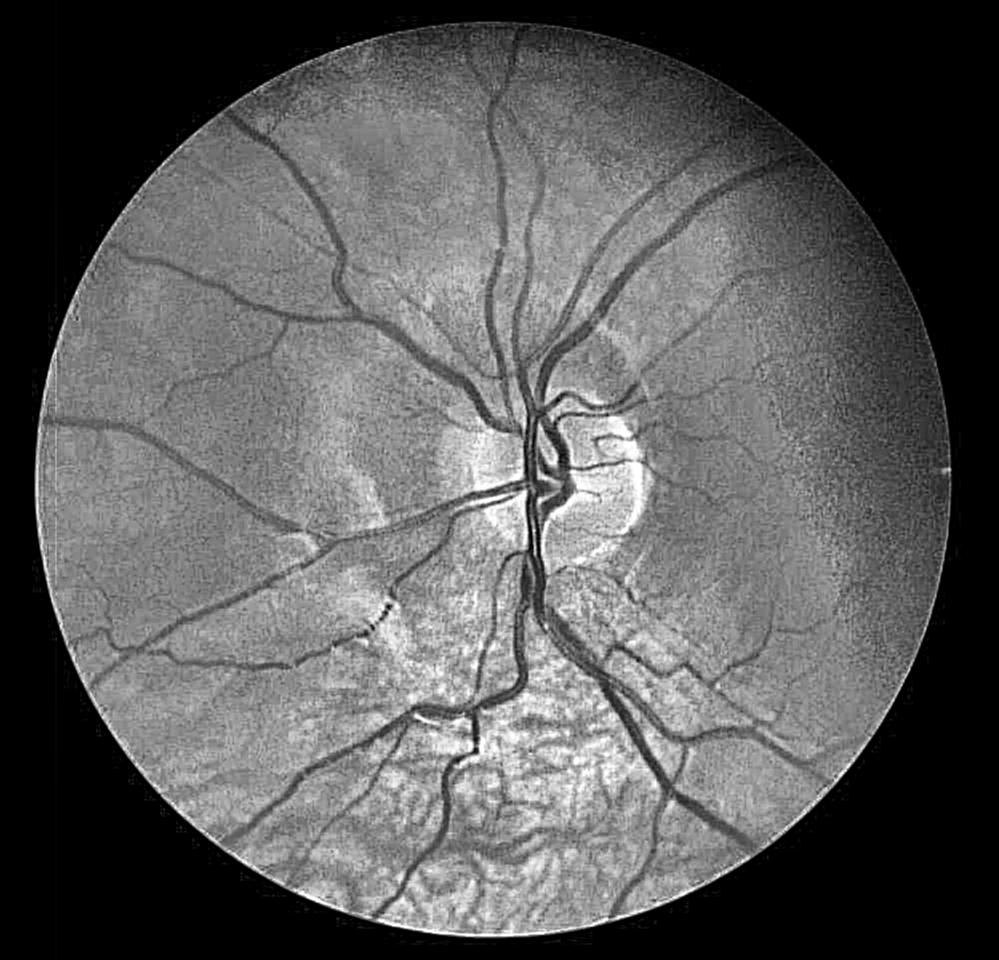
\includegraphics[width=3.6cm]{../idx0_s32_out3_x}}} &
		\bmvaHangBox{\fbox{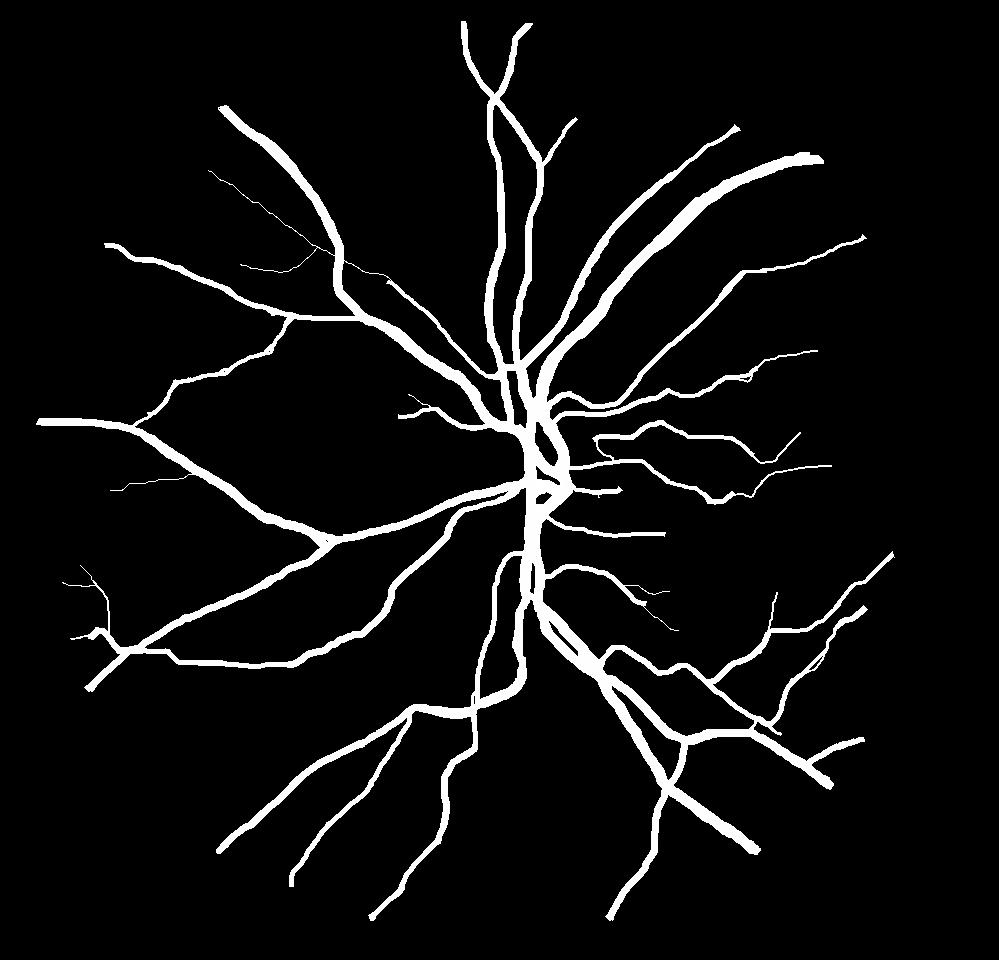
\includegraphics[width=3.6cm]{../idx0_s32_out2_y}}} &
		\bmvaHangBox{\fbox{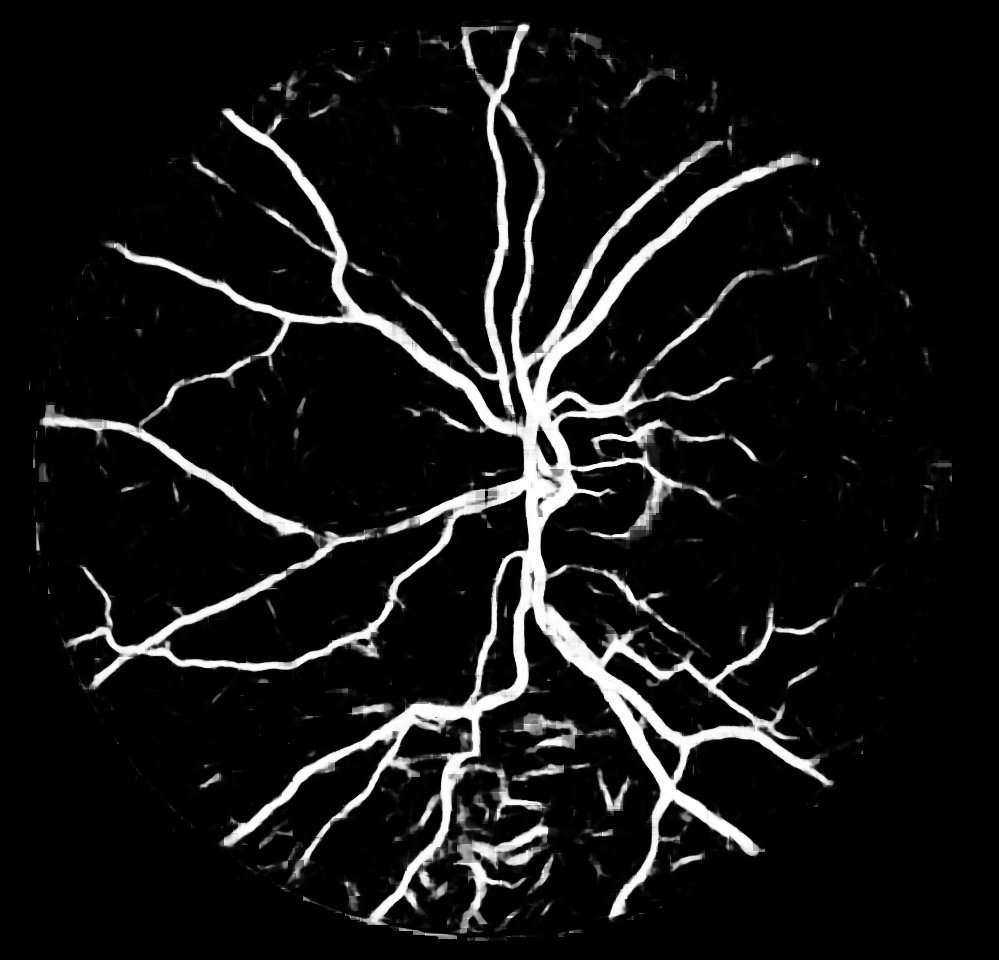
\includegraphics[width=3.6cm]{../idx0_s32_out1_p}}}\\

		\bmvaHangBox{\fbox{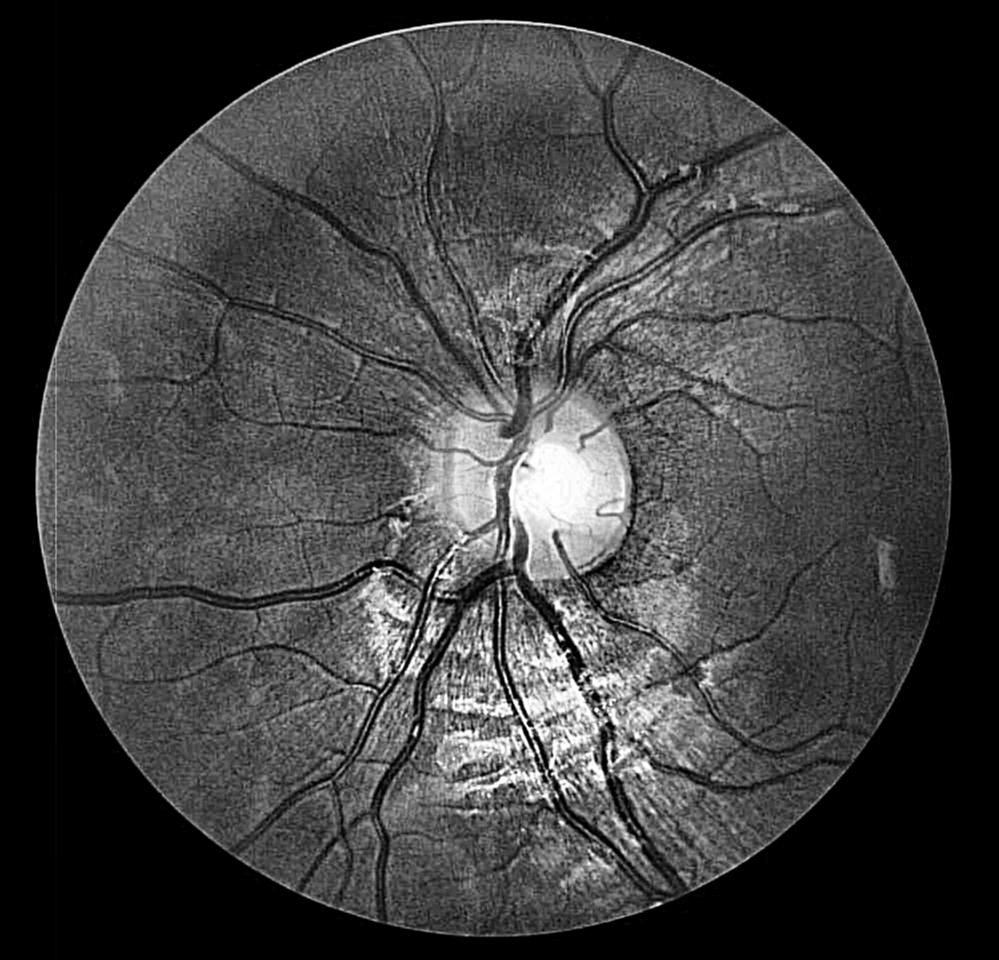
\includegraphics[width=3.6cm]{../idx1_s32_out3_x}}} &
		\bmvaHangBox{\fbox{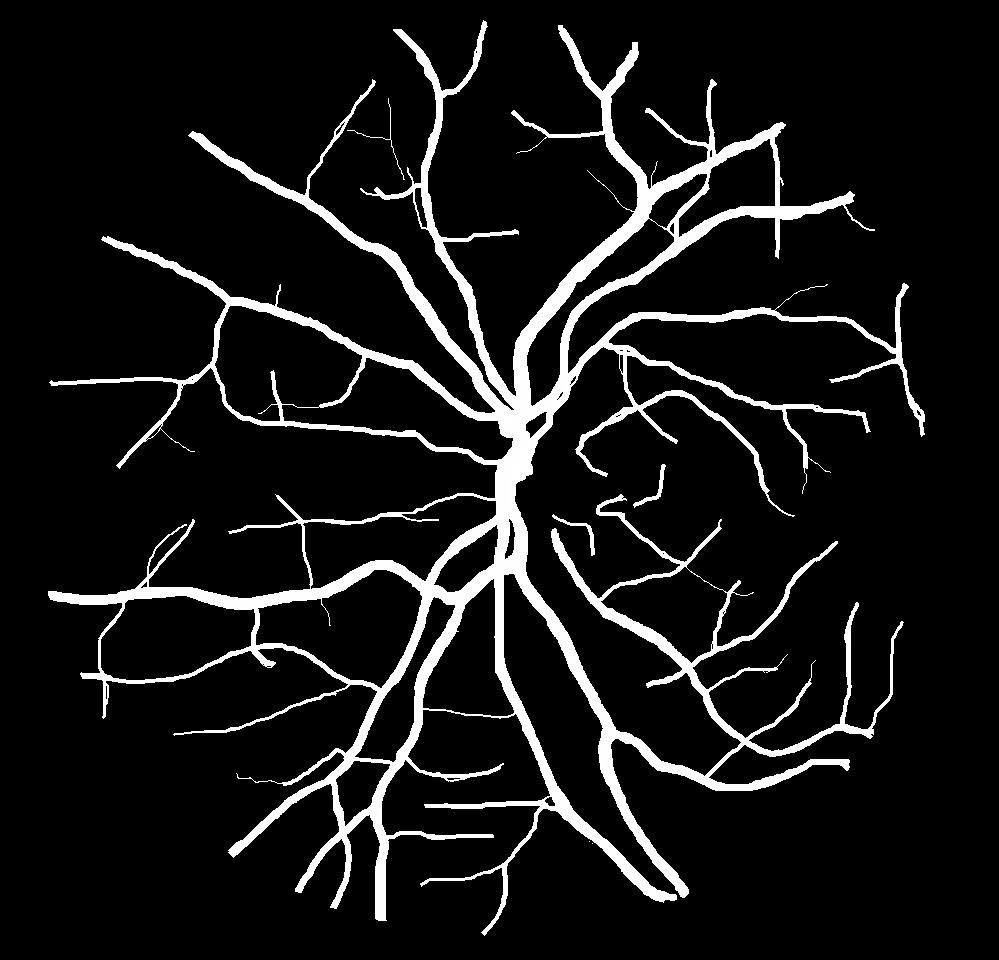
\includegraphics[width=3.6cm]{../idx1_s32_out2_y}}} &
		\bmvaHangBox{\fbox{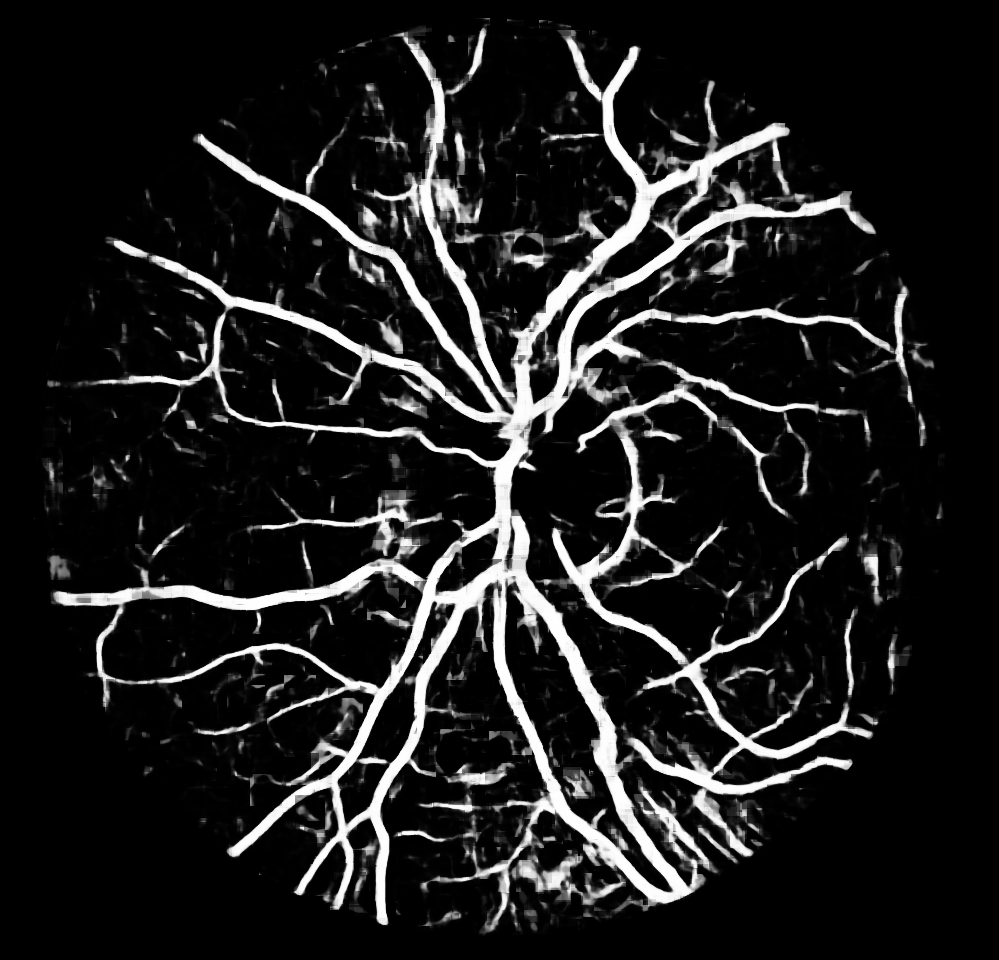
\includegraphics[width=3.6cm]{../idx1_s32_out1_p}}}\\

		\bmvaHangBox{\fbox{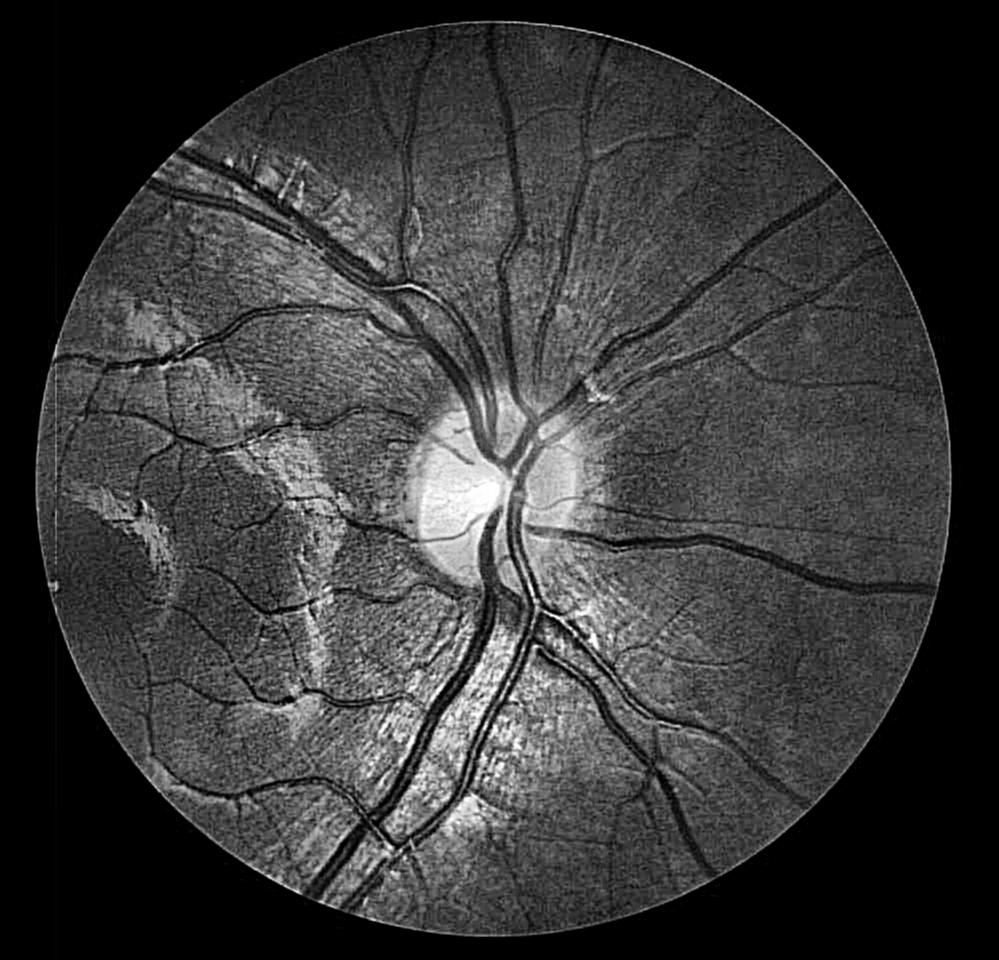
\includegraphics[width=3.6cm]{../idx2_s32_out3_x}}} &
		\bmvaHangBox{\fbox{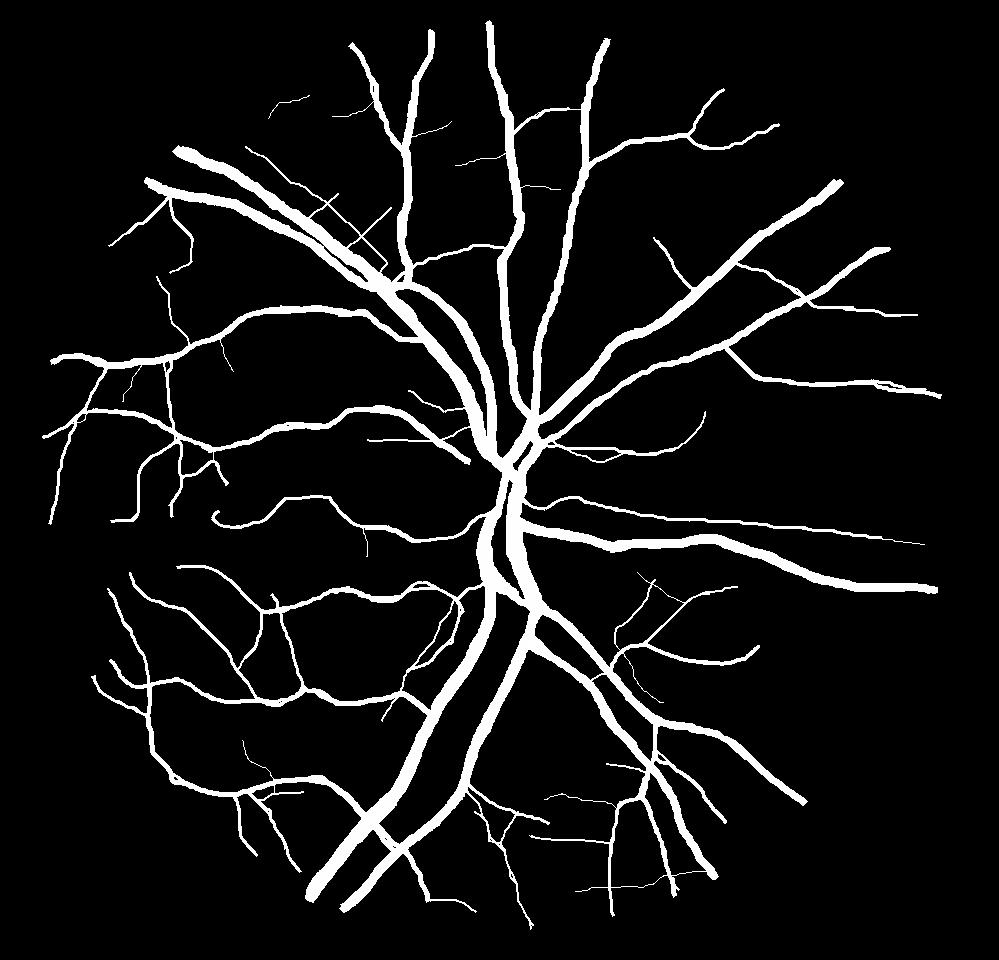
\includegraphics[width=3.6cm]{../idx2_s32_out2_y}}} &
		\bmvaHangBox{\fbox{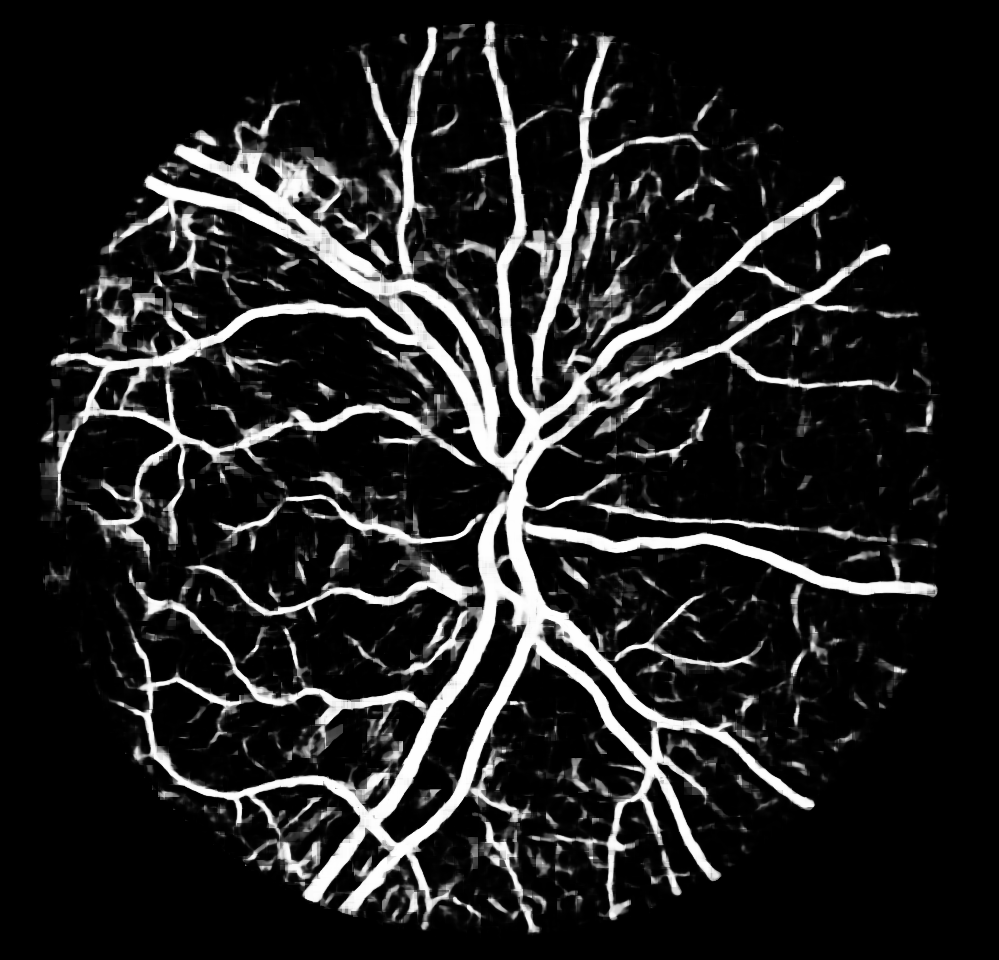
\includegraphics[width=3.6cm]{../idx2_s32_out1_p}}}\\

		\bmvaHangBox{\fbox{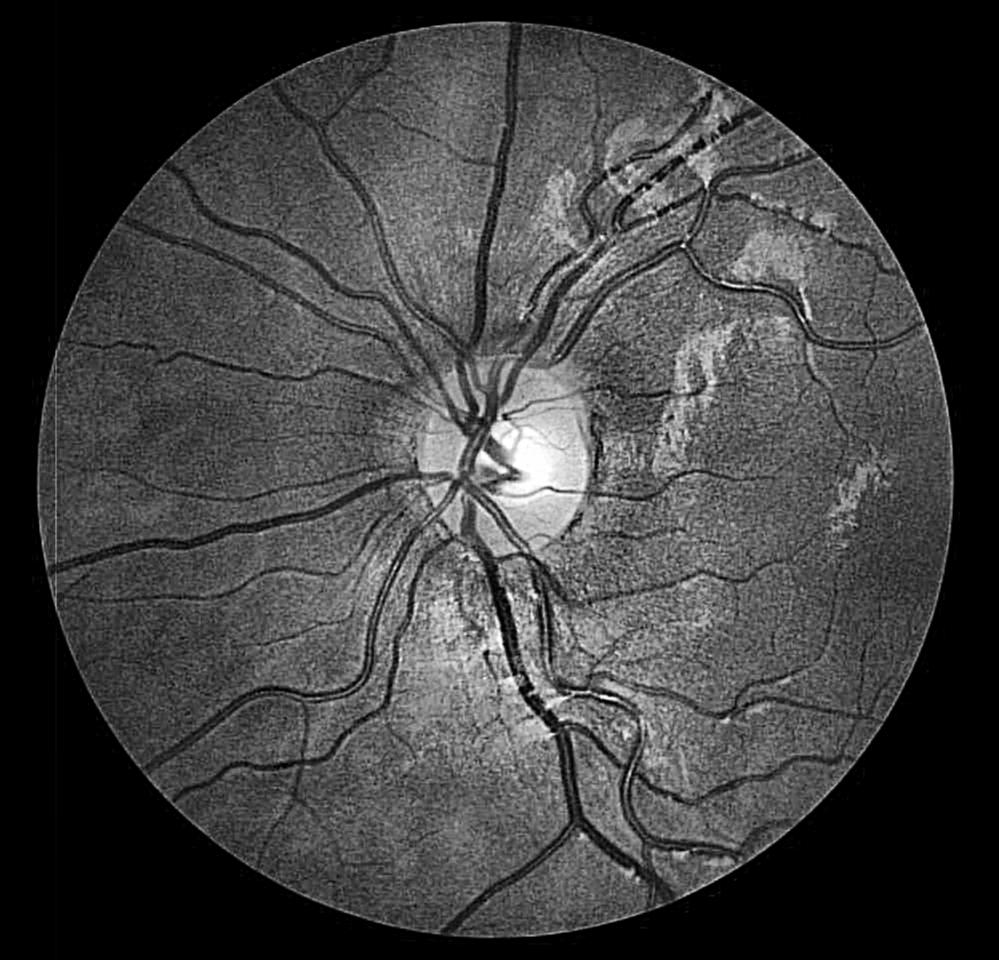
\includegraphics[width=3.6cm]{../idx3_s32_out3_x}}} &
		\bmvaHangBox{\fbox{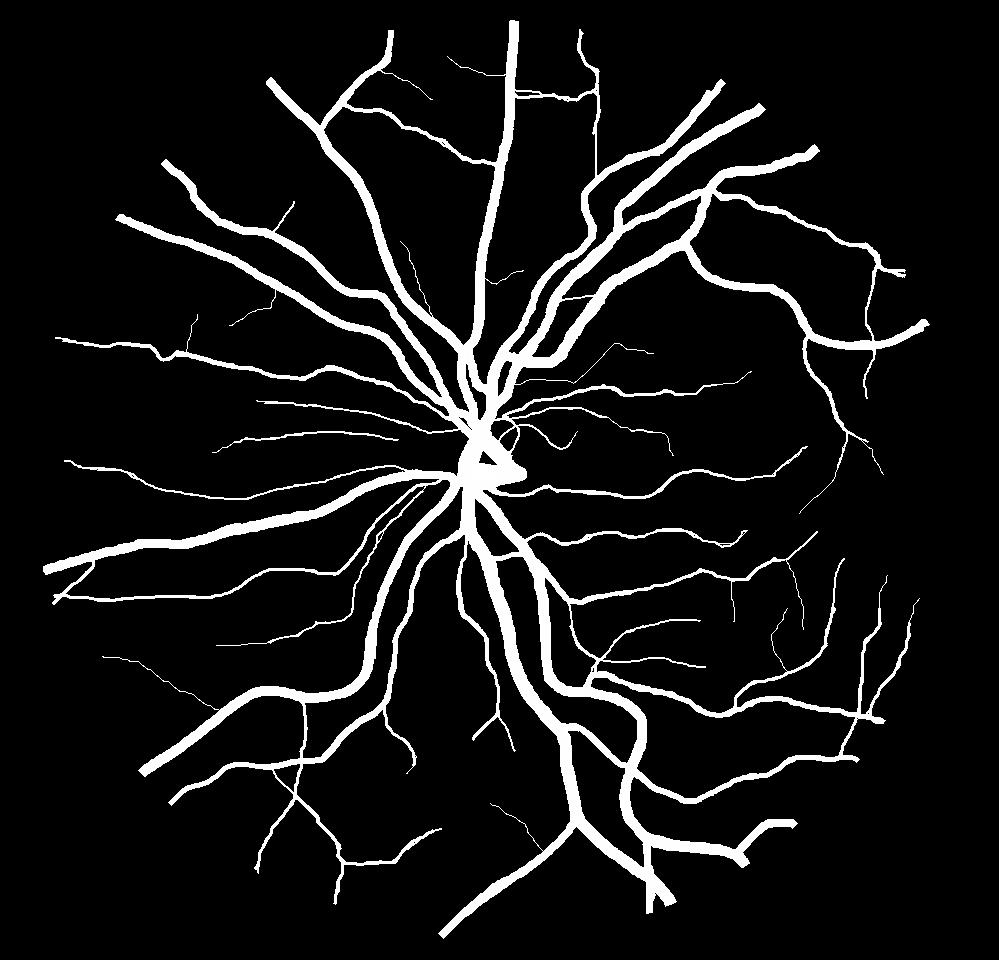
\includegraphics[width=3.6cm]{../idx3_s32_out2_y}}} &
		\bmvaHangBox{\fbox{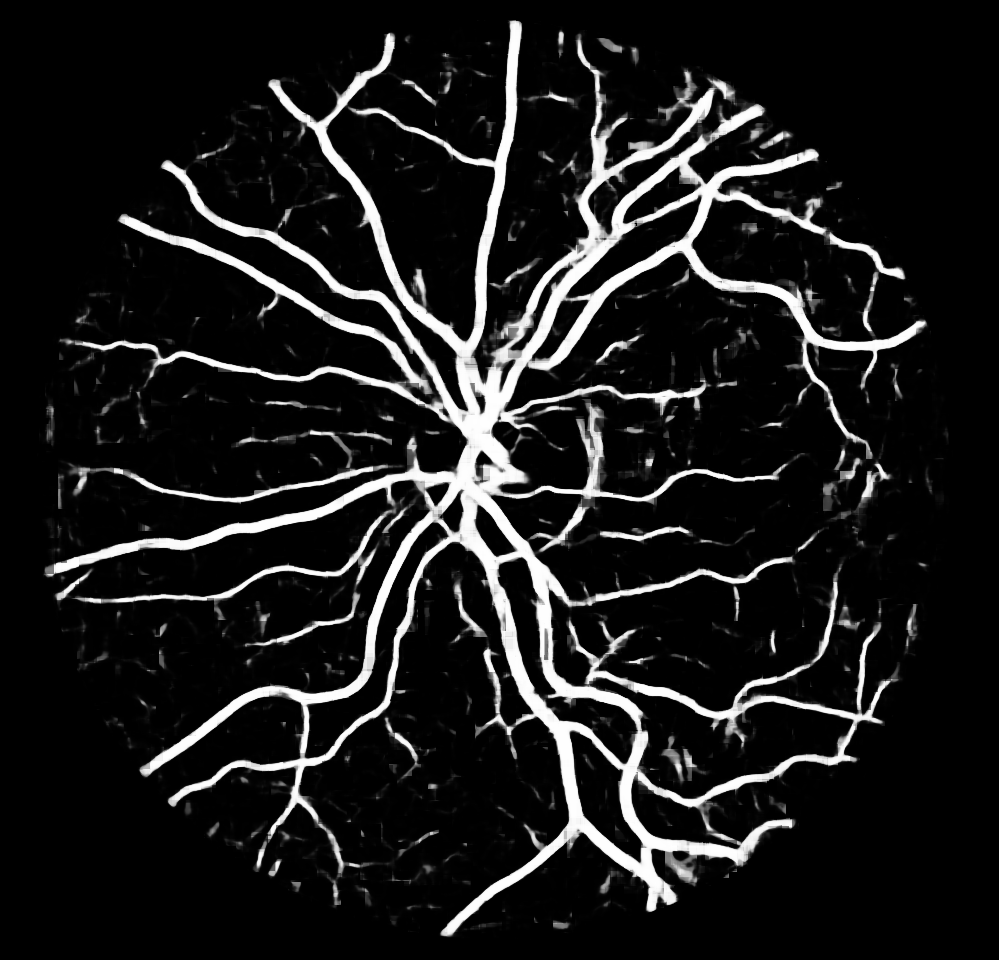
\includegraphics[width=3.6cm]{../idx3_s32_out1_p}}}\\

		\bmvaHangBox{\fbox{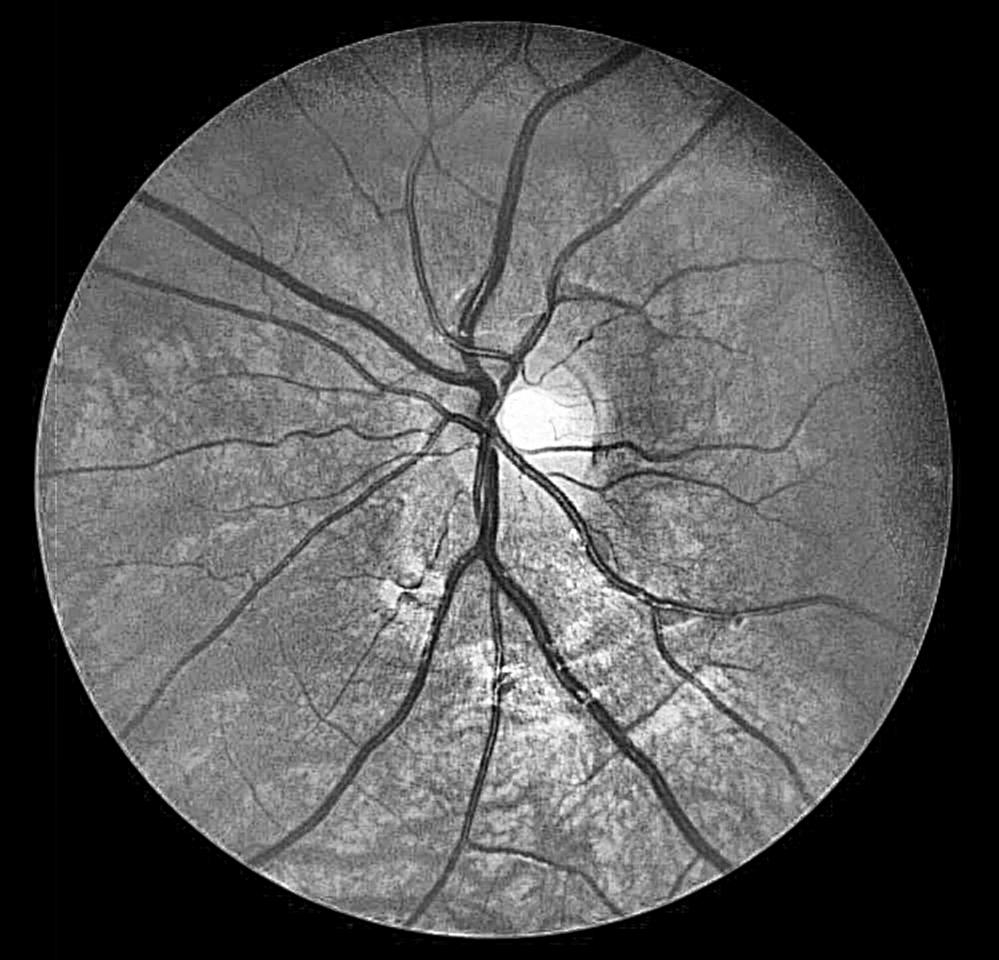
\includegraphics[width=3.6cm]{../idx4_s32_out3_x}}} &
		\bmvaHangBox{\fbox{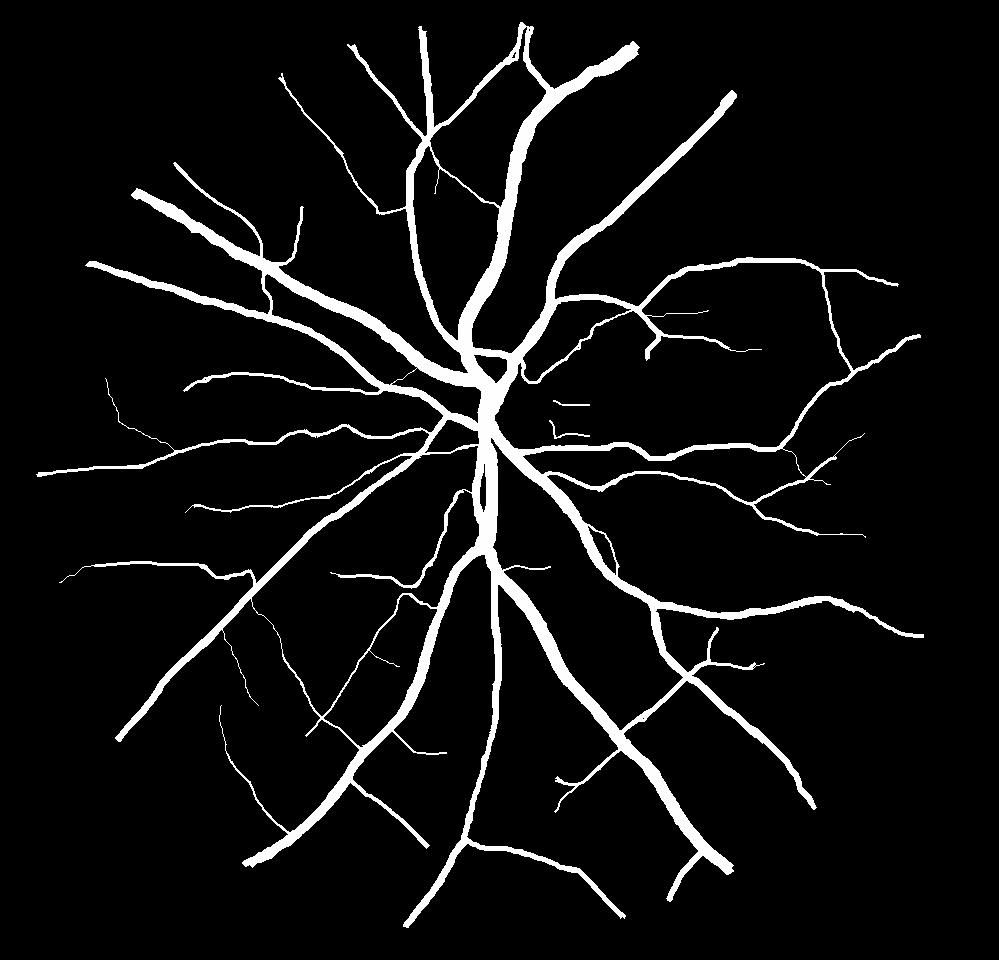
\includegraphics[width=3.6cm]{../idx4_s32_out2_y}}} &
		\bmvaHangBox{\fbox{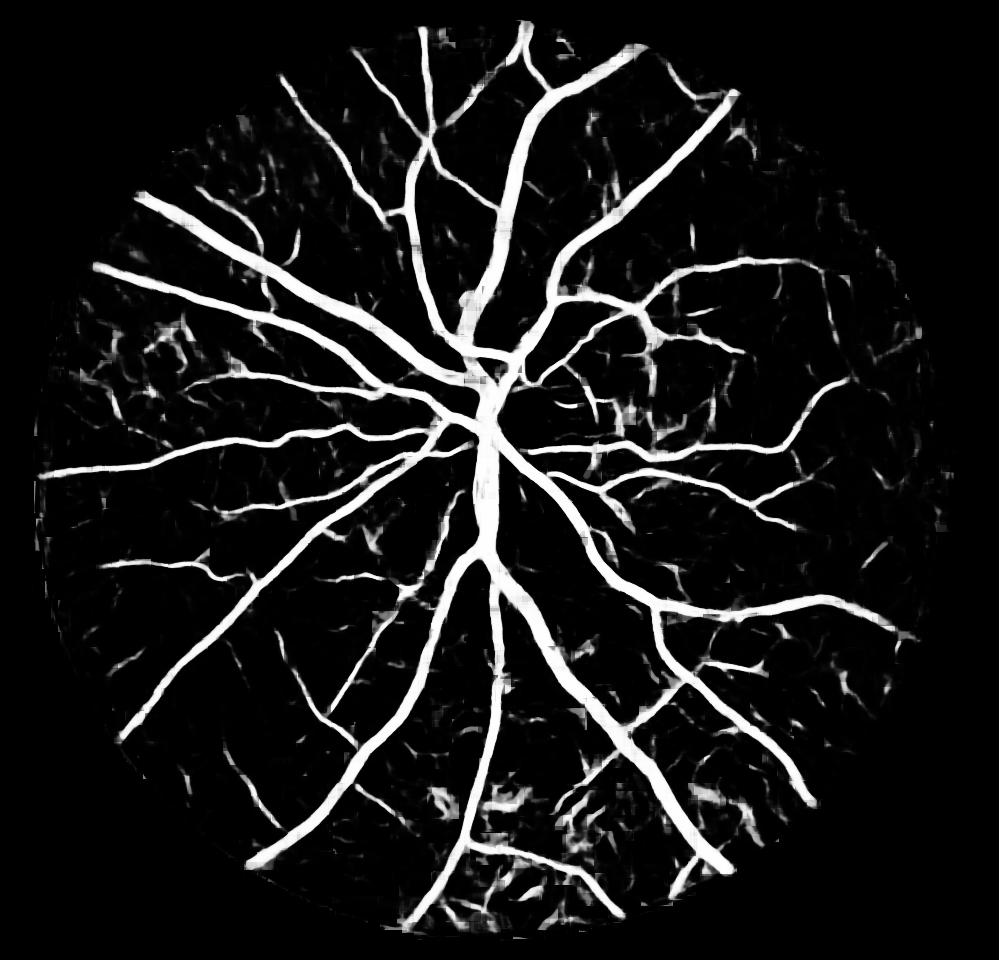
\includegraphics[width=3.6cm]{../idx4_s32_out1_p}}}\\

		(input)&(gt)&(pred)
\end{tabular}
\caption{Dla detektora 32x32px.}
\end{figure}


\begin{figure}[H]
	\begin{tabular}{ccc}
		\bmvaHangBox{\fbox{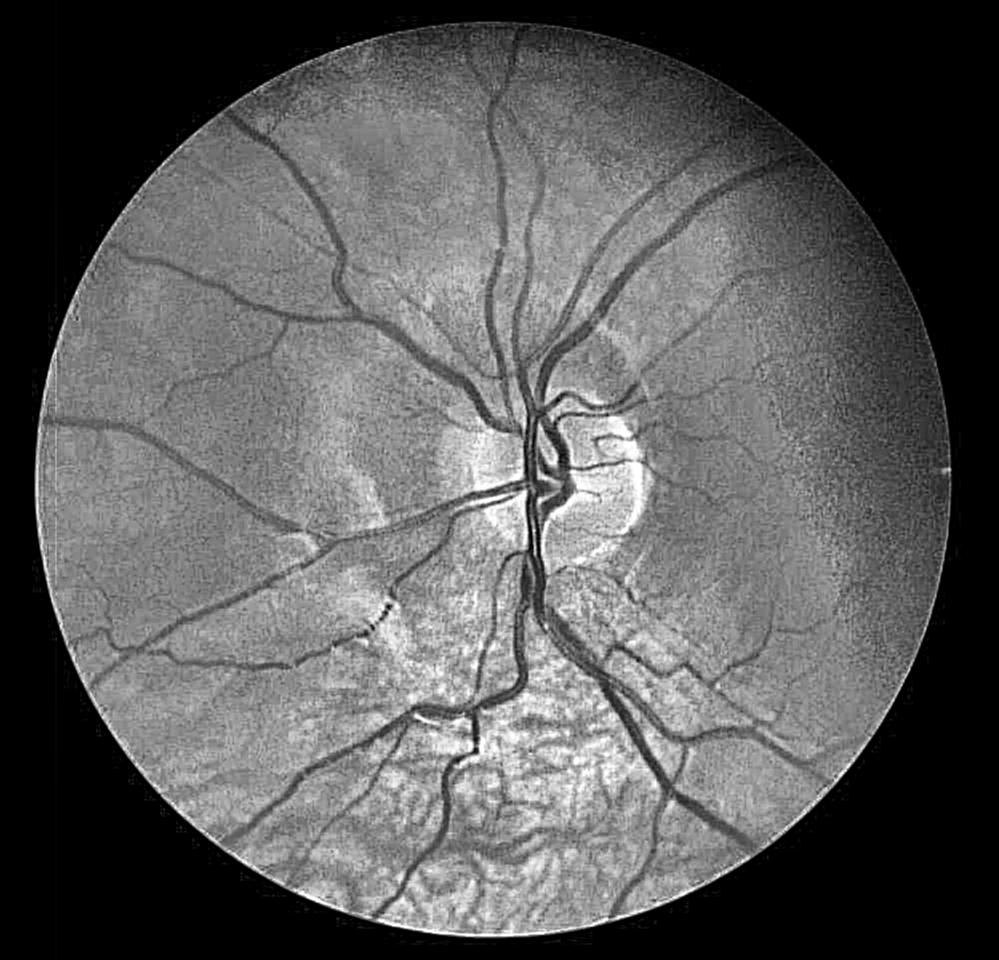
\includegraphics[width=3.6cm]{../idx0_s48_out3_x}}} &
		\bmvaHangBox{\fbox{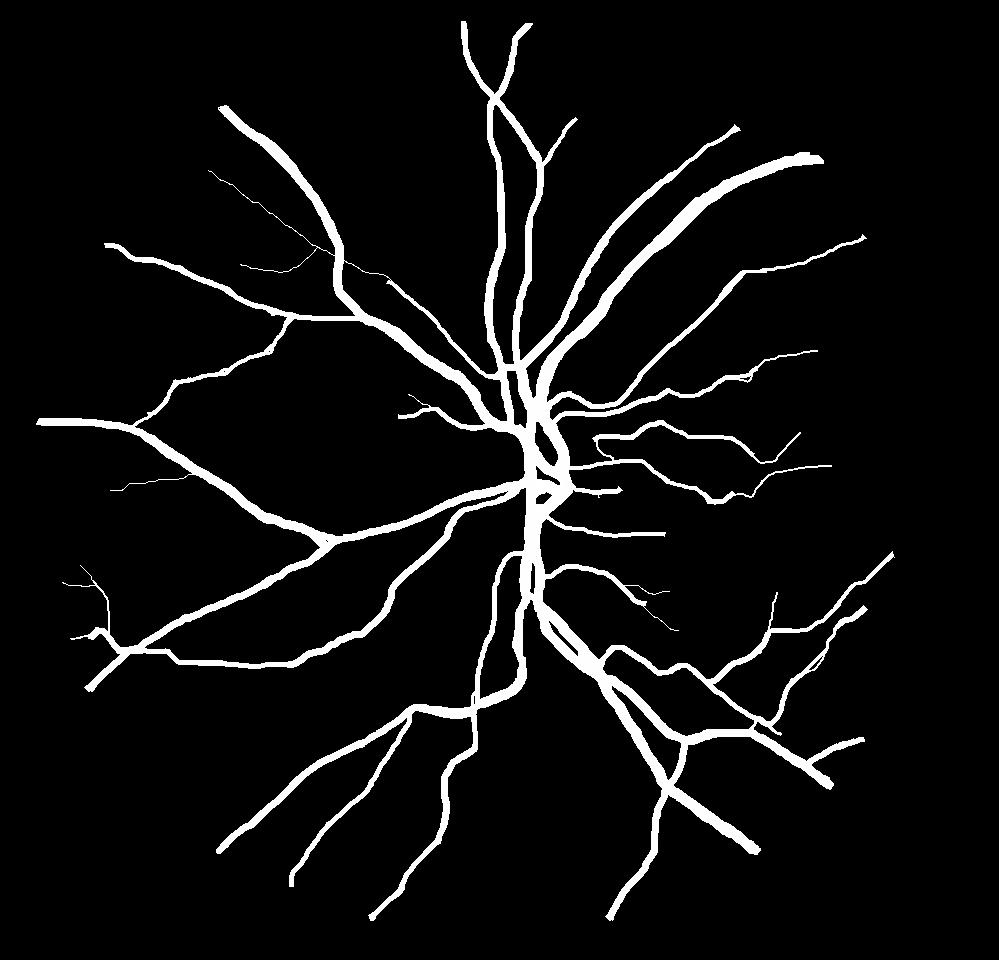
\includegraphics[width=3.6cm]{../idx0_s48_out2_y}}} &
		\bmvaHangBox{\fbox{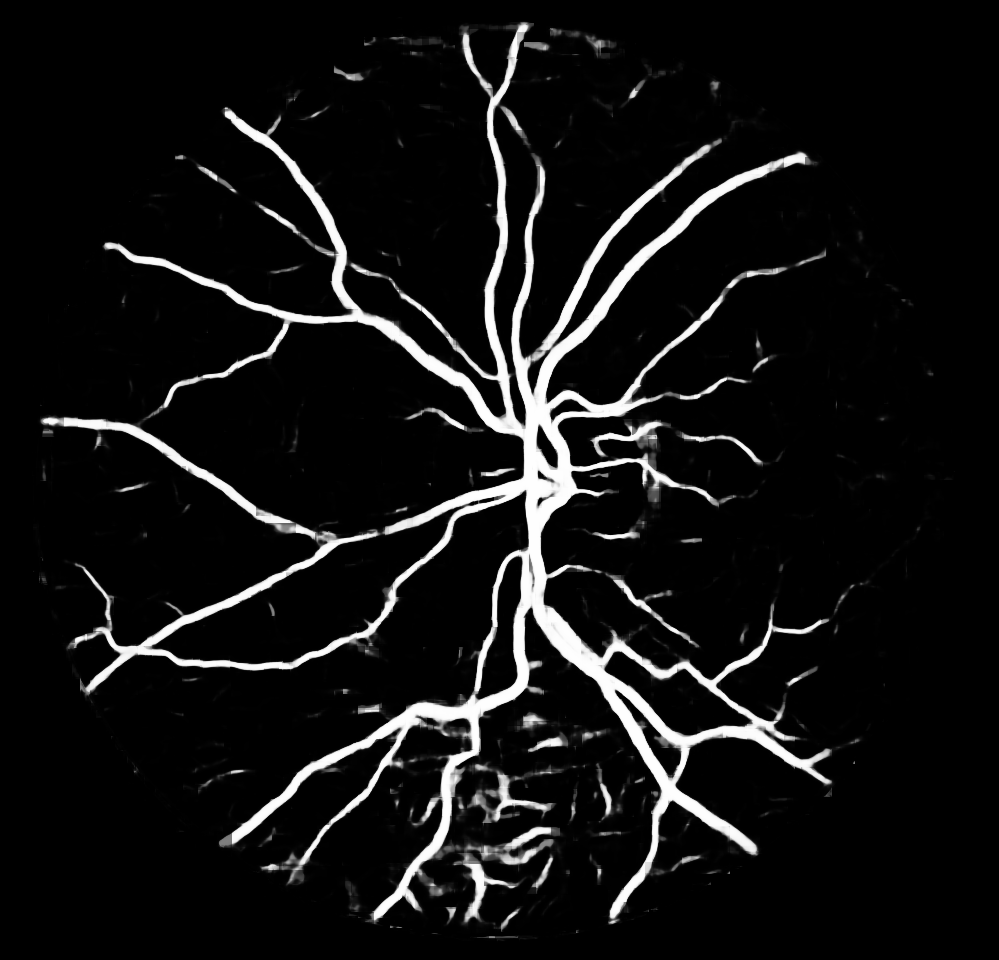
\includegraphics[width=3.6cm]{../idx0_s48_out1_p}}}\\

		\bmvaHangBox{\fbox{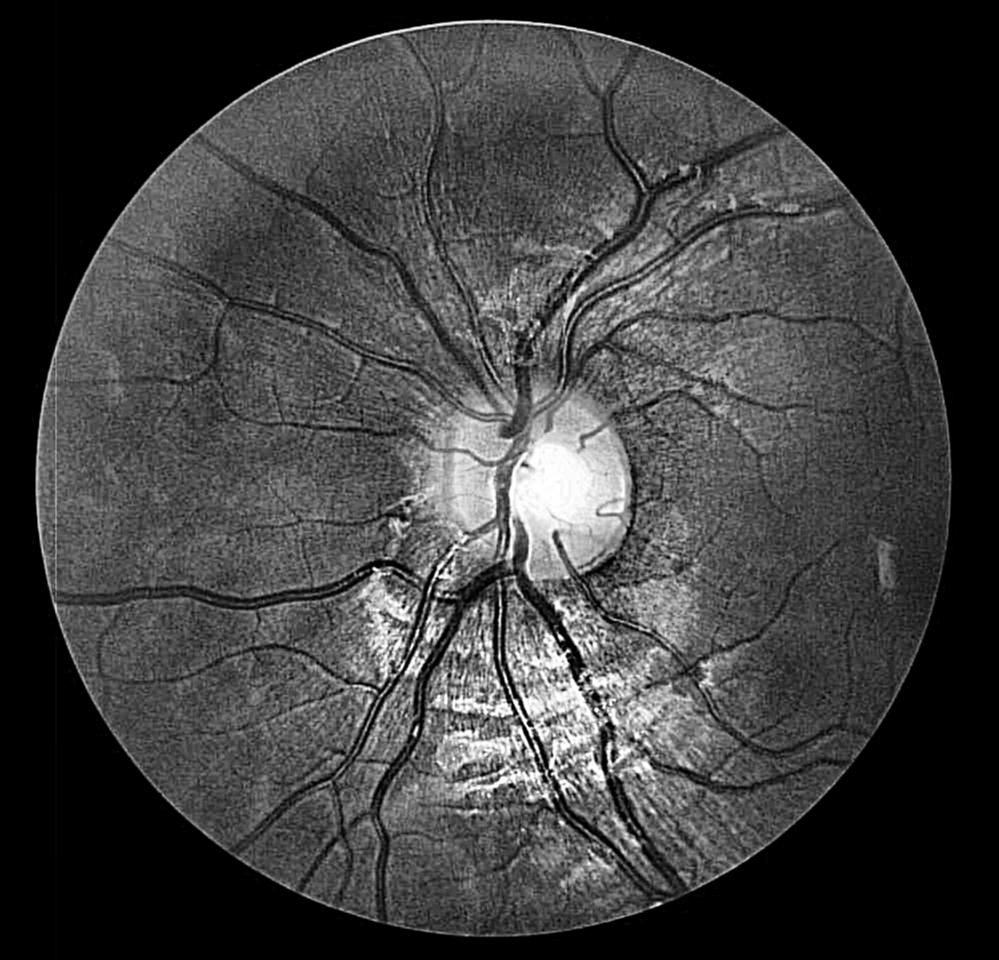
\includegraphics[width=3.6cm]{../idx1_s48_out3_x}}} &
		\bmvaHangBox{\fbox{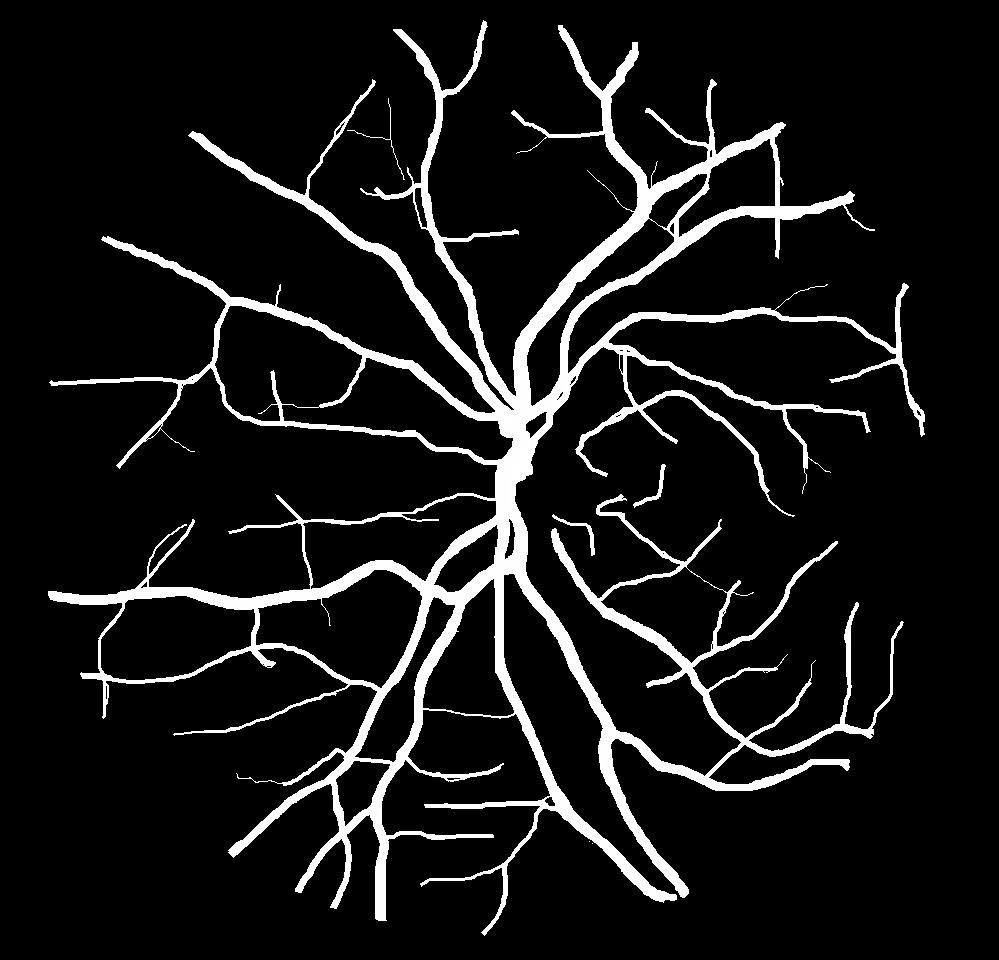
\includegraphics[width=3.6cm]{../idx1_s48_out2_y}}} &
		\bmvaHangBox{\fbox{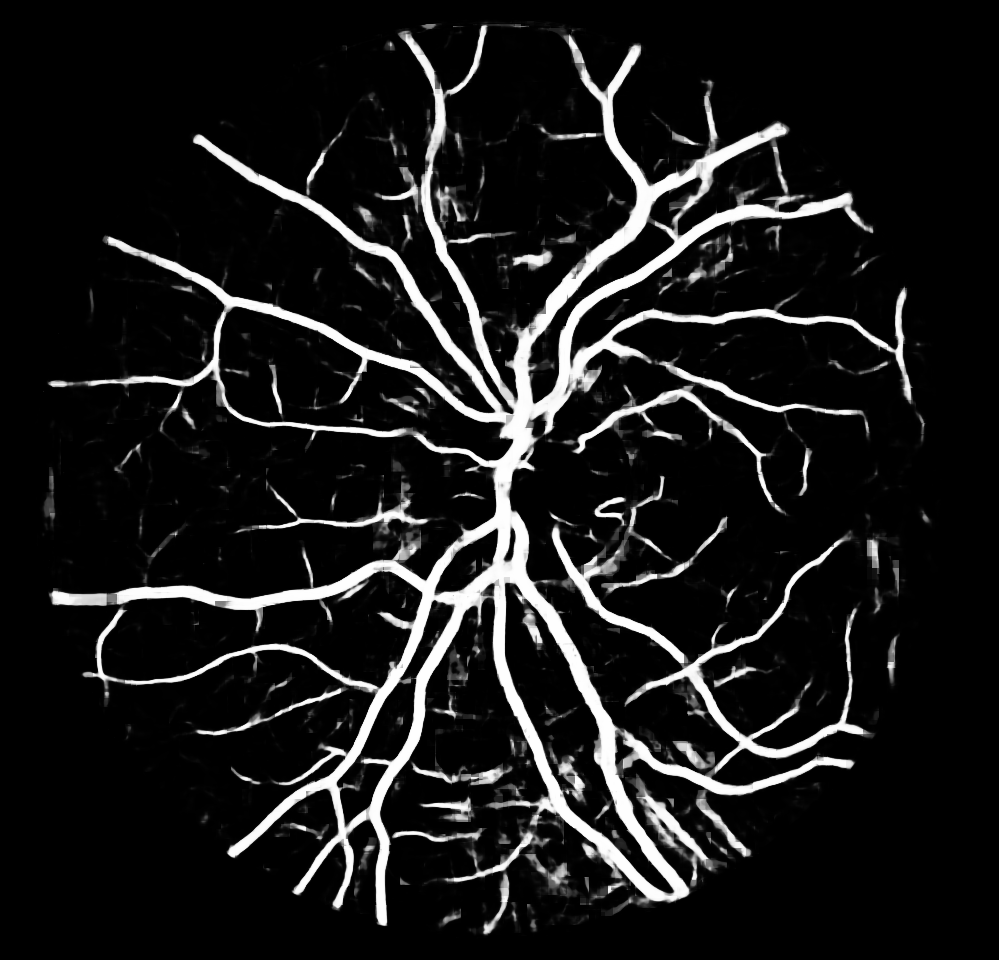
\includegraphics[width=3.6cm]{../idx1_s48_out1_p}}}\\

		\bmvaHangBox{\fbox{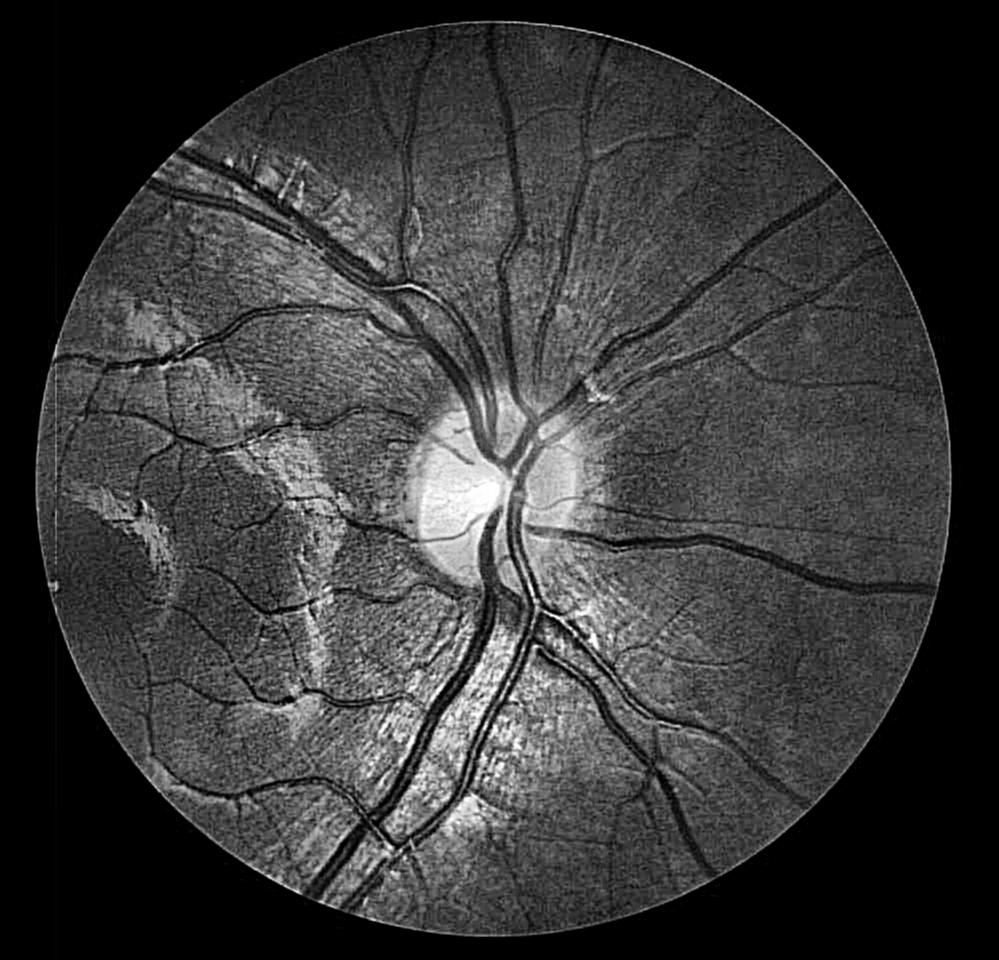
\includegraphics[width=3.6cm]{../idx2_s48_out3_x}}} &
		\bmvaHangBox{\fbox{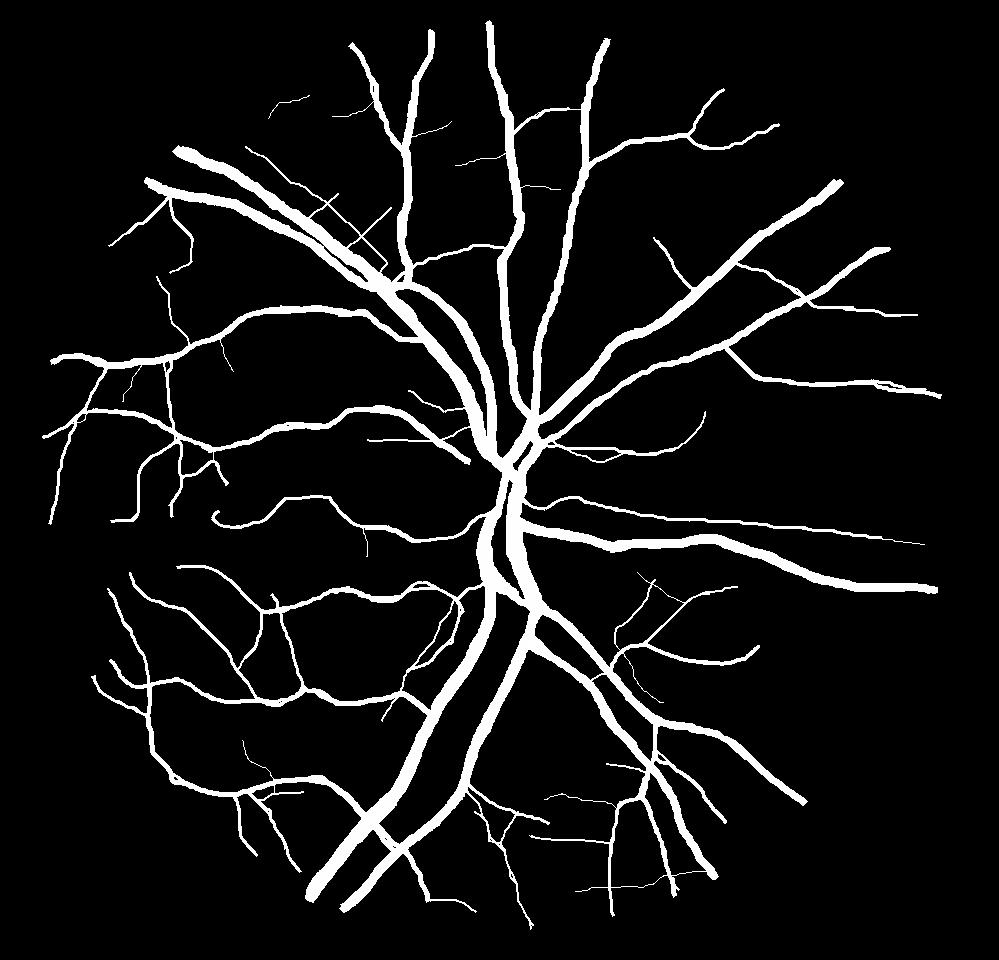
\includegraphics[width=3.6cm]{../idx2_s48_out2_y}}} &
		\bmvaHangBox{\fbox{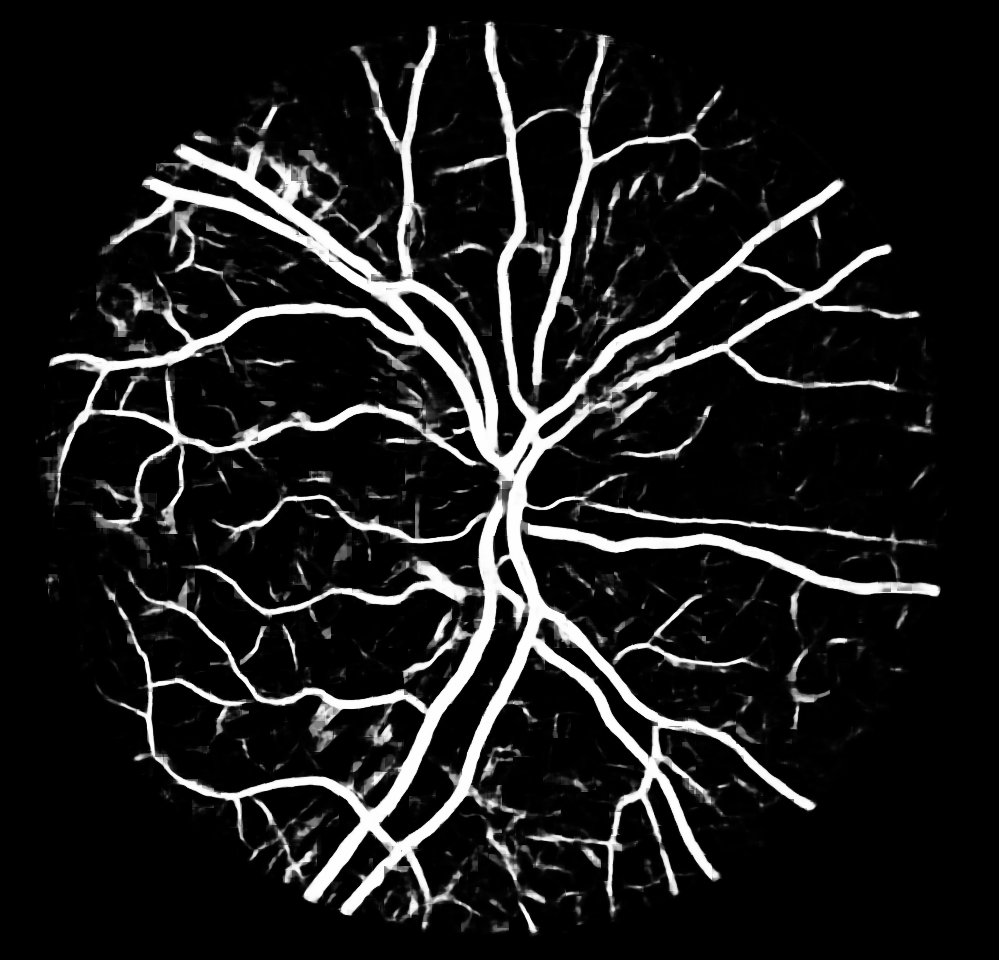
\includegraphics[width=3.6cm]{../idx2_s48_out1_p}}}\\

		\bmvaHangBox{\fbox{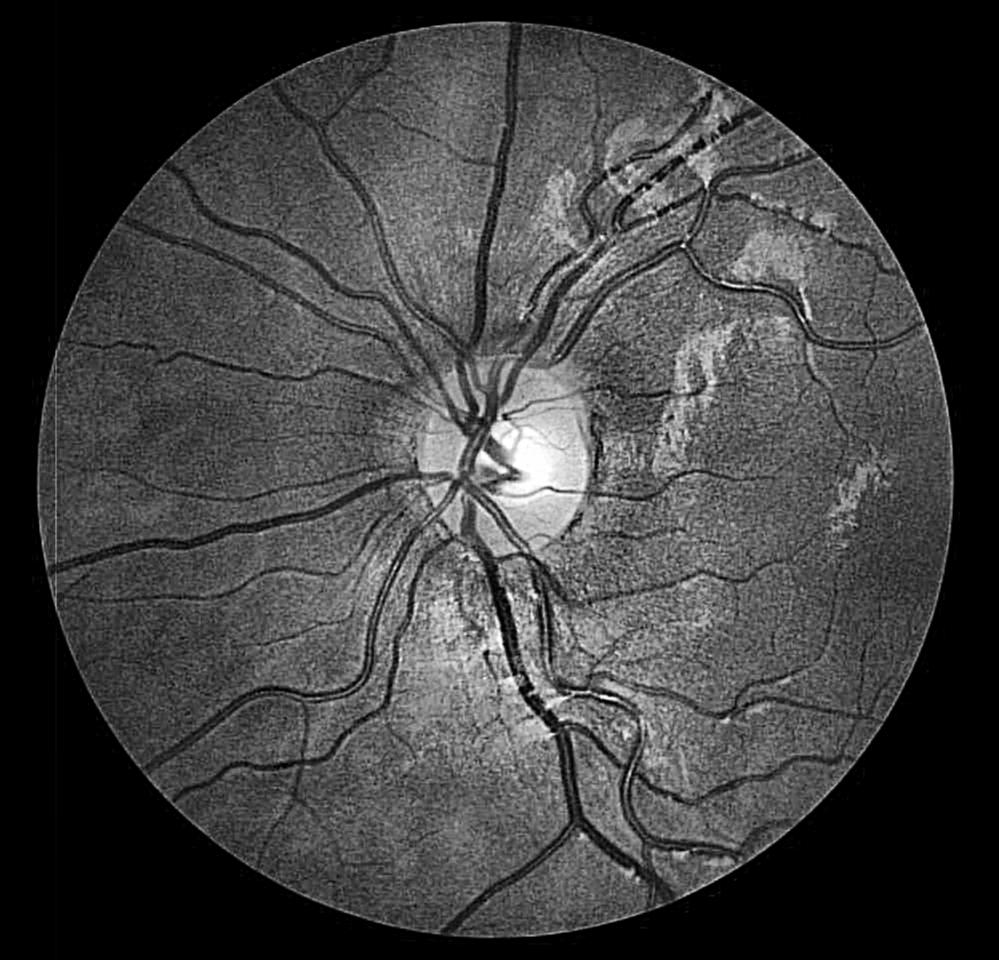
\includegraphics[width=3.6cm]{../idx3_s48_out3_x}}} &
		\bmvaHangBox{\fbox{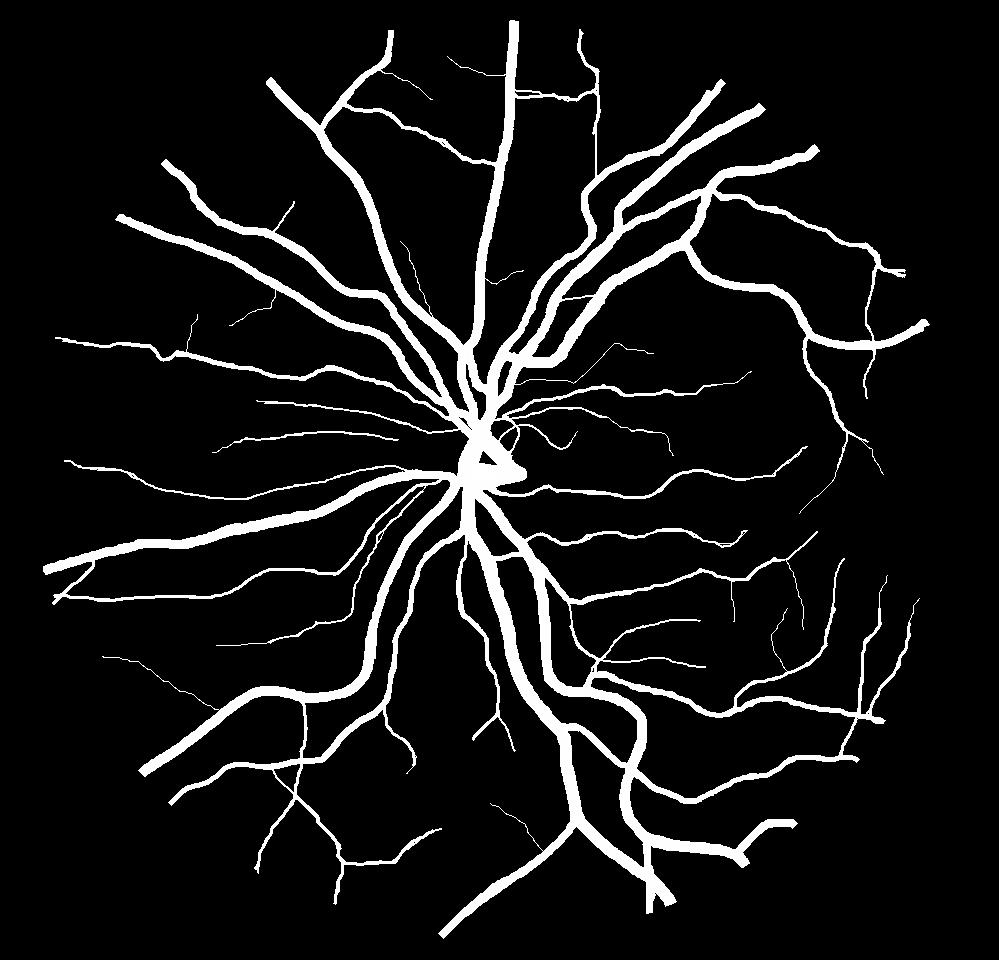
\includegraphics[width=3.6cm]{../idx3_s48_out2_y}}} &
		\bmvaHangBox{\fbox{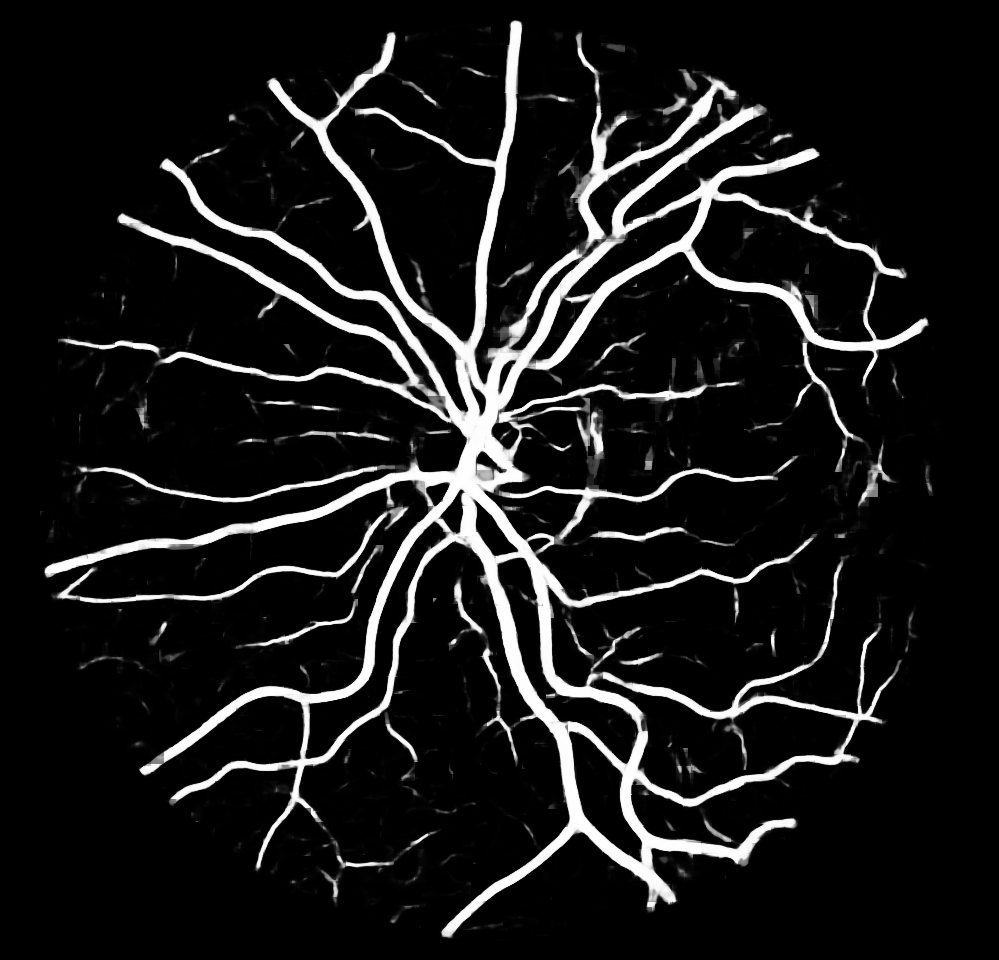
\includegraphics[width=3.6cm]{../idx3_s48_out1_p}}}\\

		\bmvaHangBox{\fbox{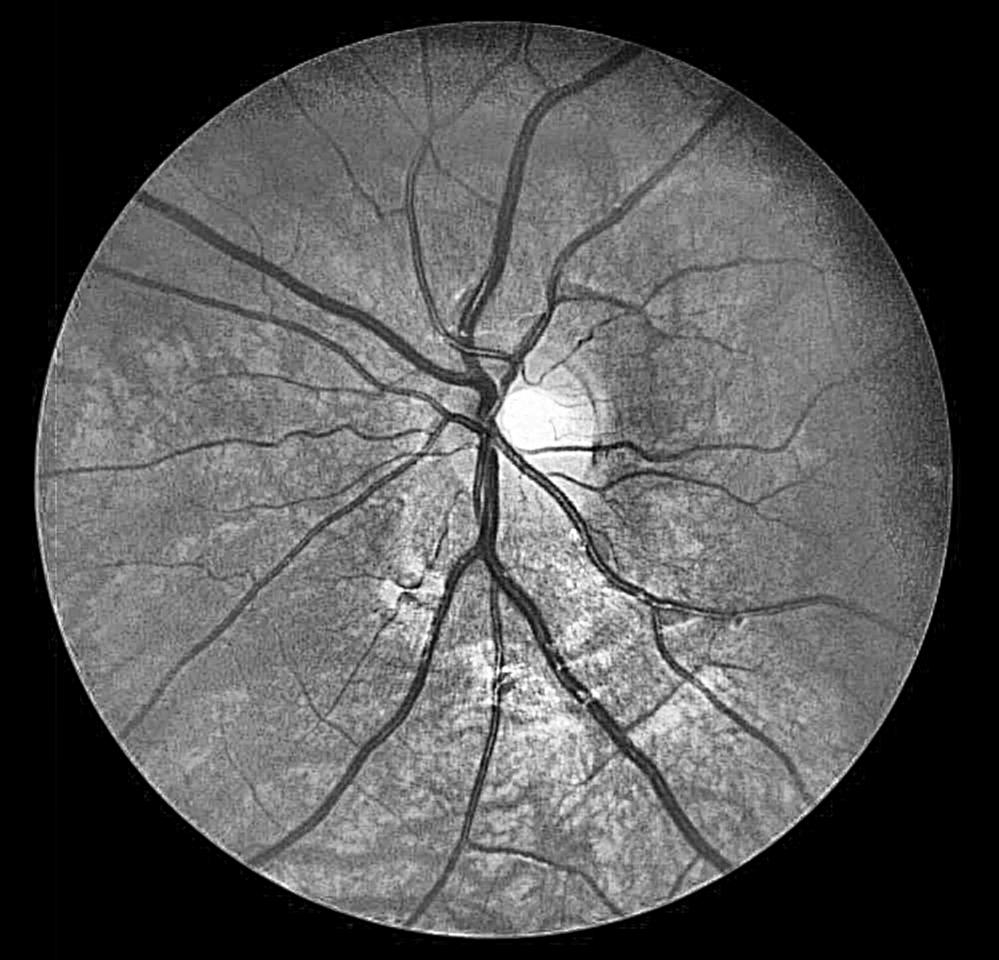
\includegraphics[width=3.6cm]{../idx4_s48_out3_x}}} &
		\bmvaHangBox{\fbox{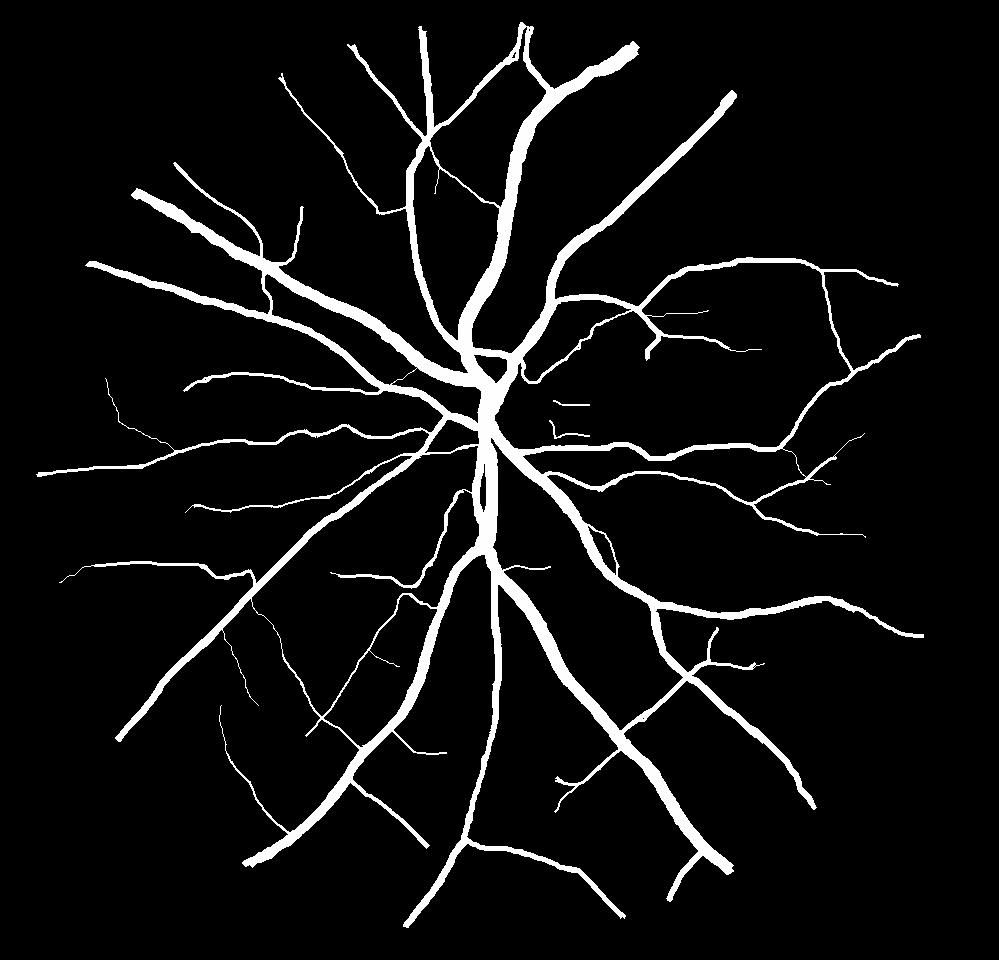
\includegraphics[width=3.6cm]{../idx4_s48_out2_y}}} &
		\bmvaHangBox{\fbox{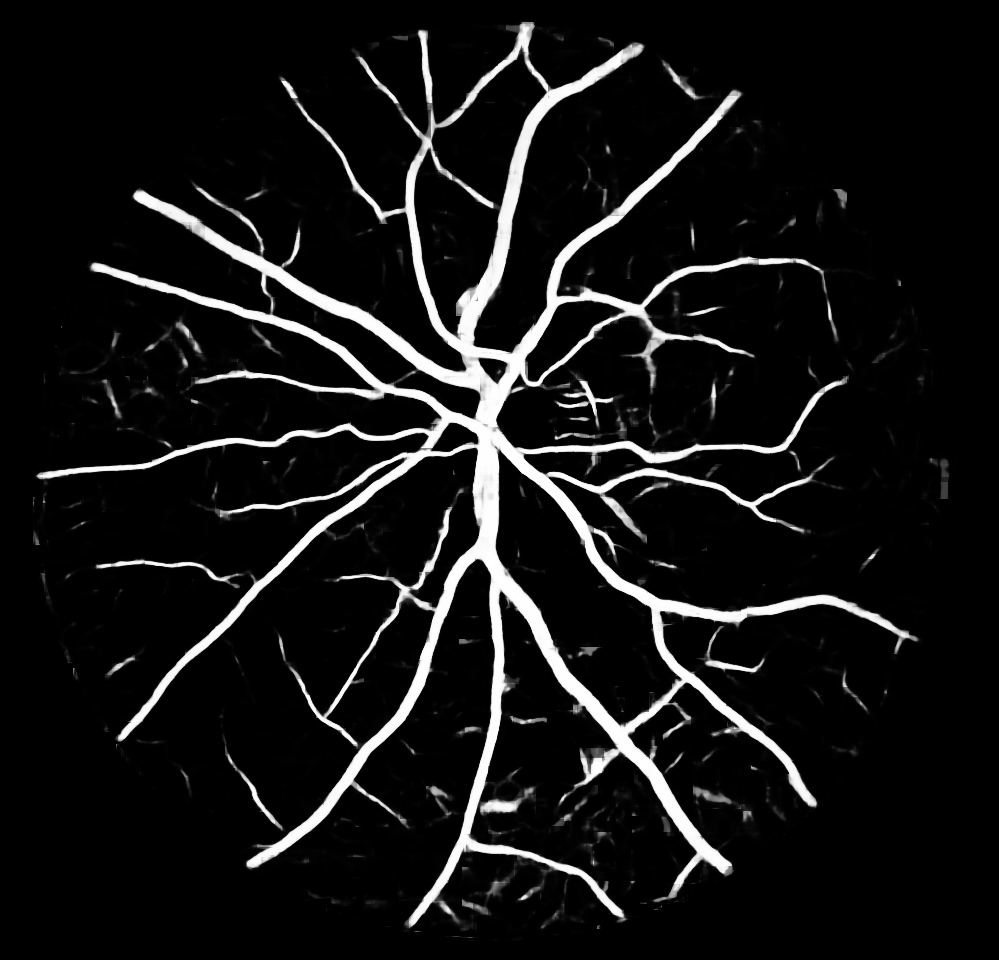
\includegraphics[width=3.6cm]{../idx4_s48_out1_p}}}\\

		(input)&(gt)&(pred)
\end{tabular}
\caption{Dla detektora 48x48px.}
\end{figure}


\begin{figure}[H]
	\begin{tabular}{ccc}
		\bmvaHangBox{\fbox{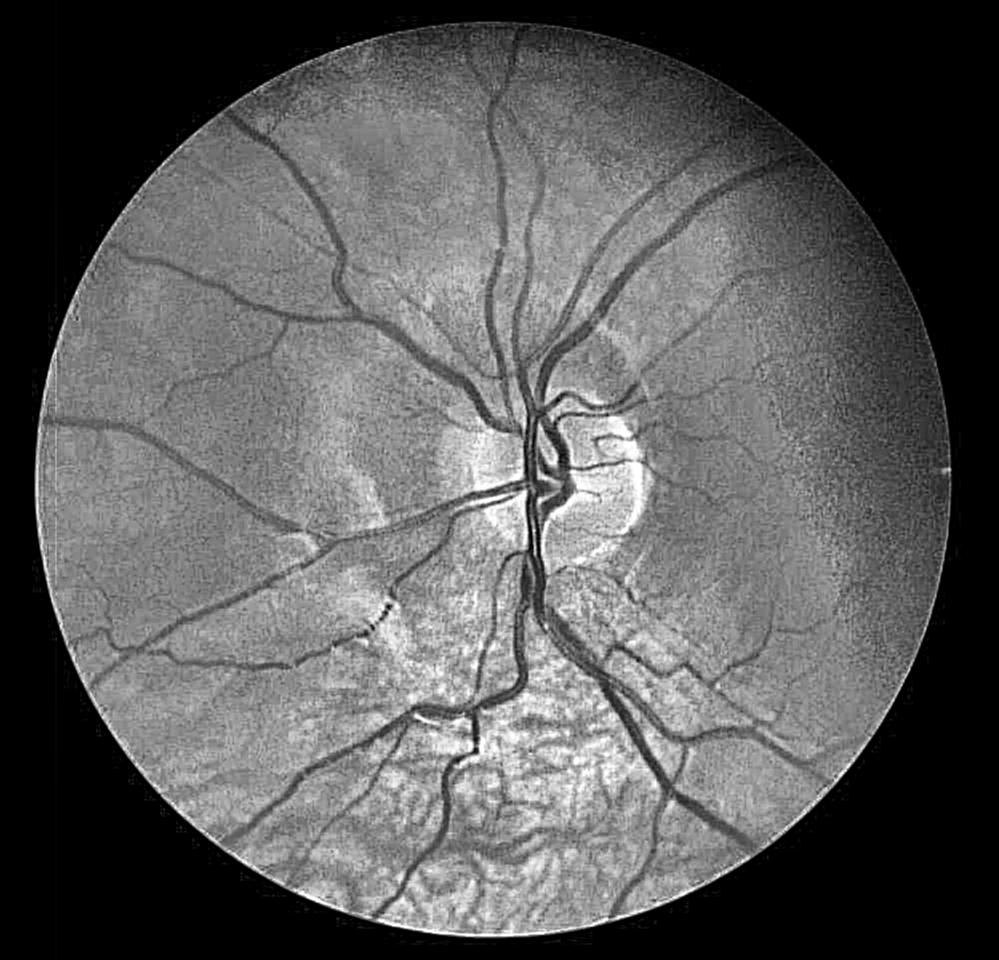
\includegraphics[width=3.6cm]{../idx0_s64_out3_x}}} &
		\bmvaHangBox{\fbox{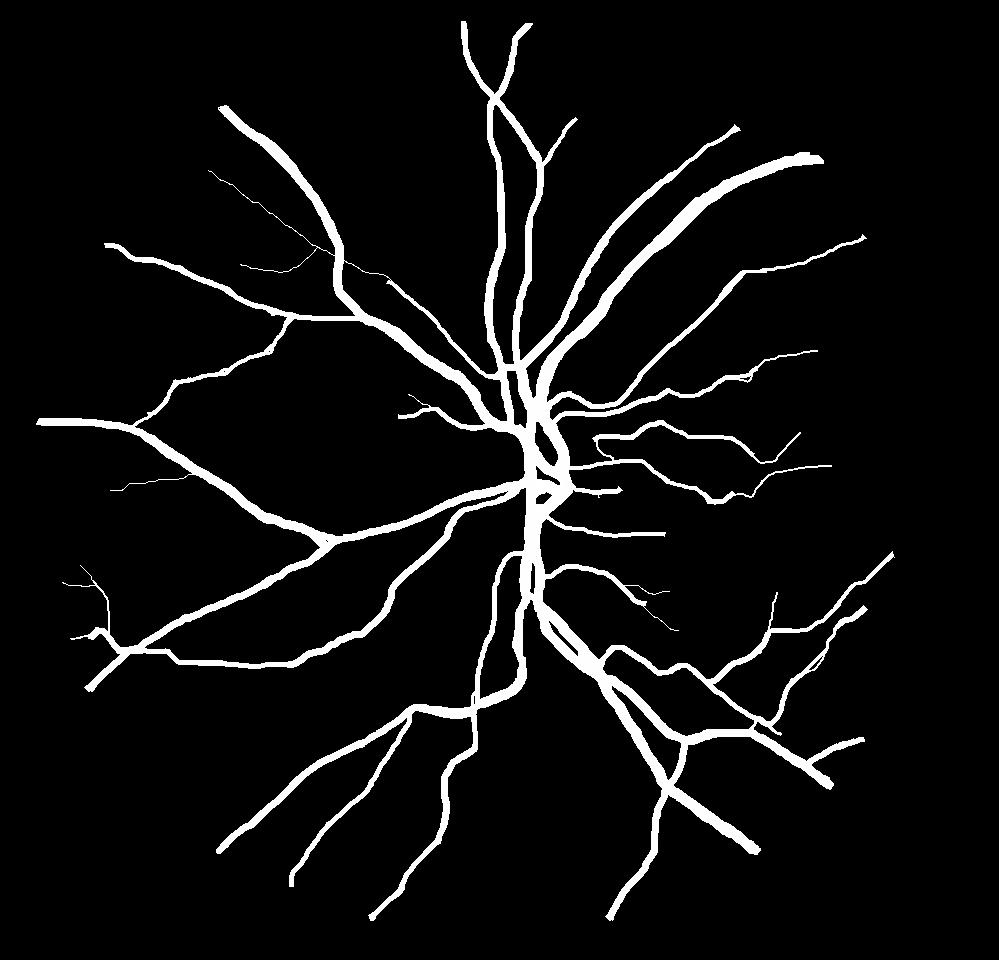
\includegraphics[width=3.6cm]{../idx0_s64_out2_y}}} &
		\bmvaHangBox{\fbox{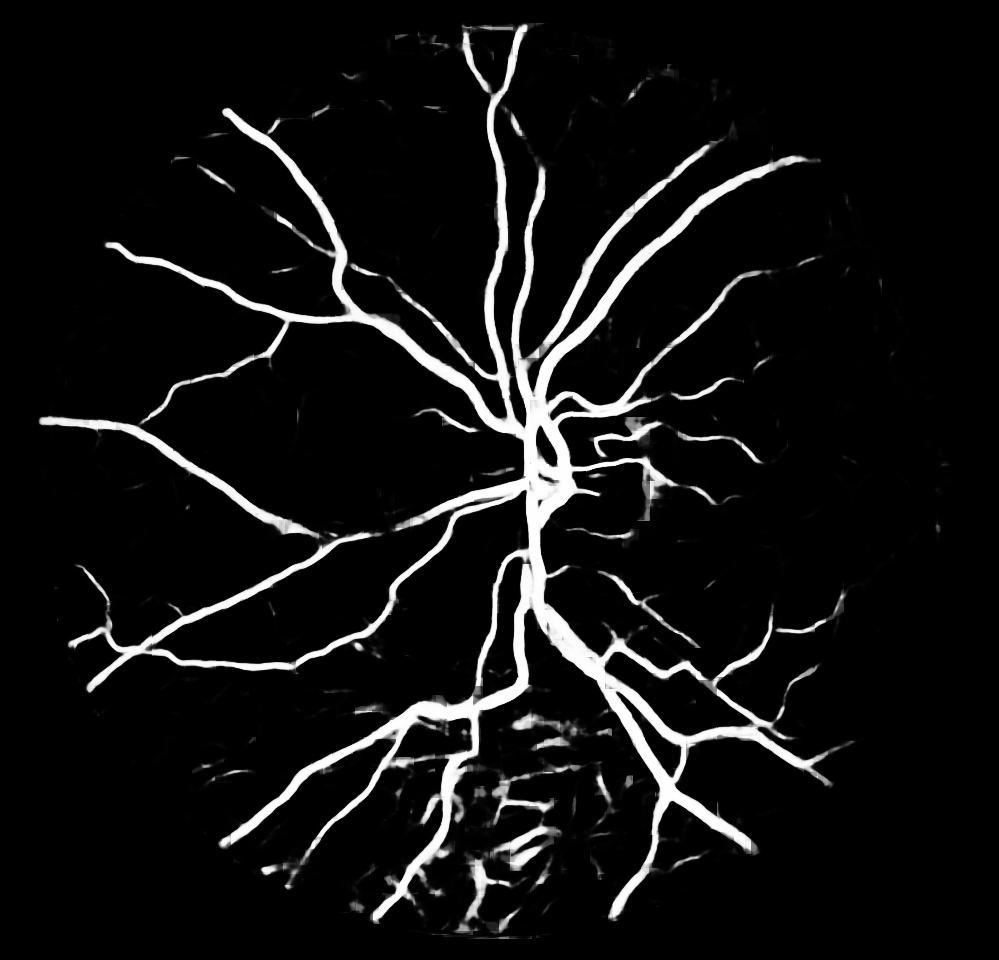
\includegraphics[width=3.6cm]{../idx0_s64_out1_p}}}\\

		\bmvaHangBox{\fbox{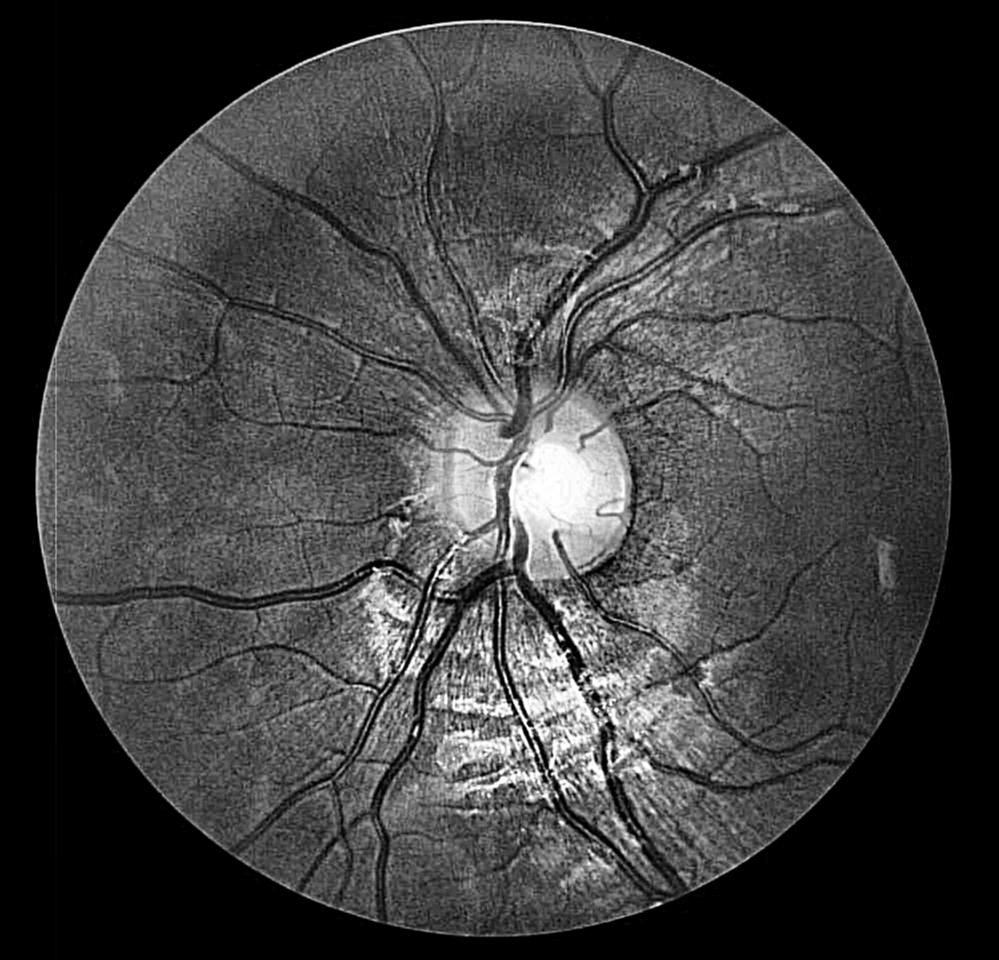
\includegraphics[width=3.6cm]{../idx1_s64_out3_x}}} &
		\bmvaHangBox{\fbox{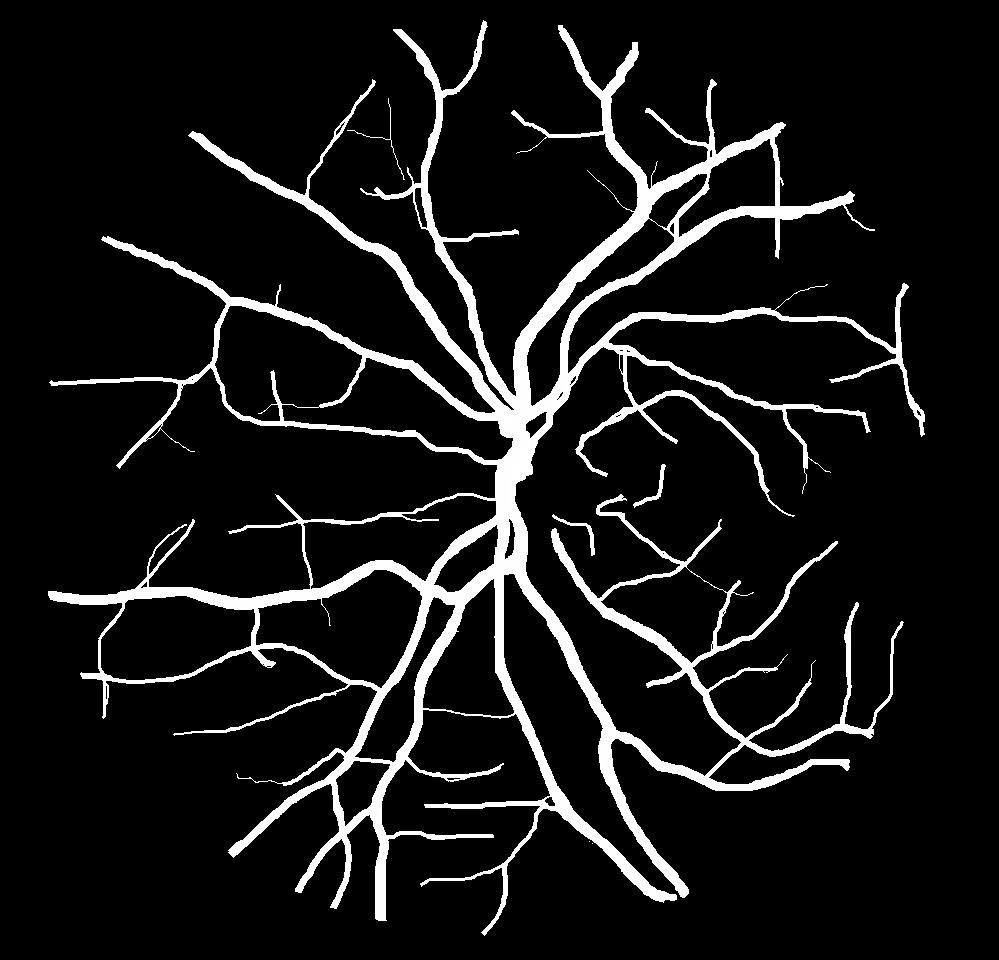
\includegraphics[width=3.6cm]{../idx1_s64_out2_y}}} &
		\bmvaHangBox{\fbox{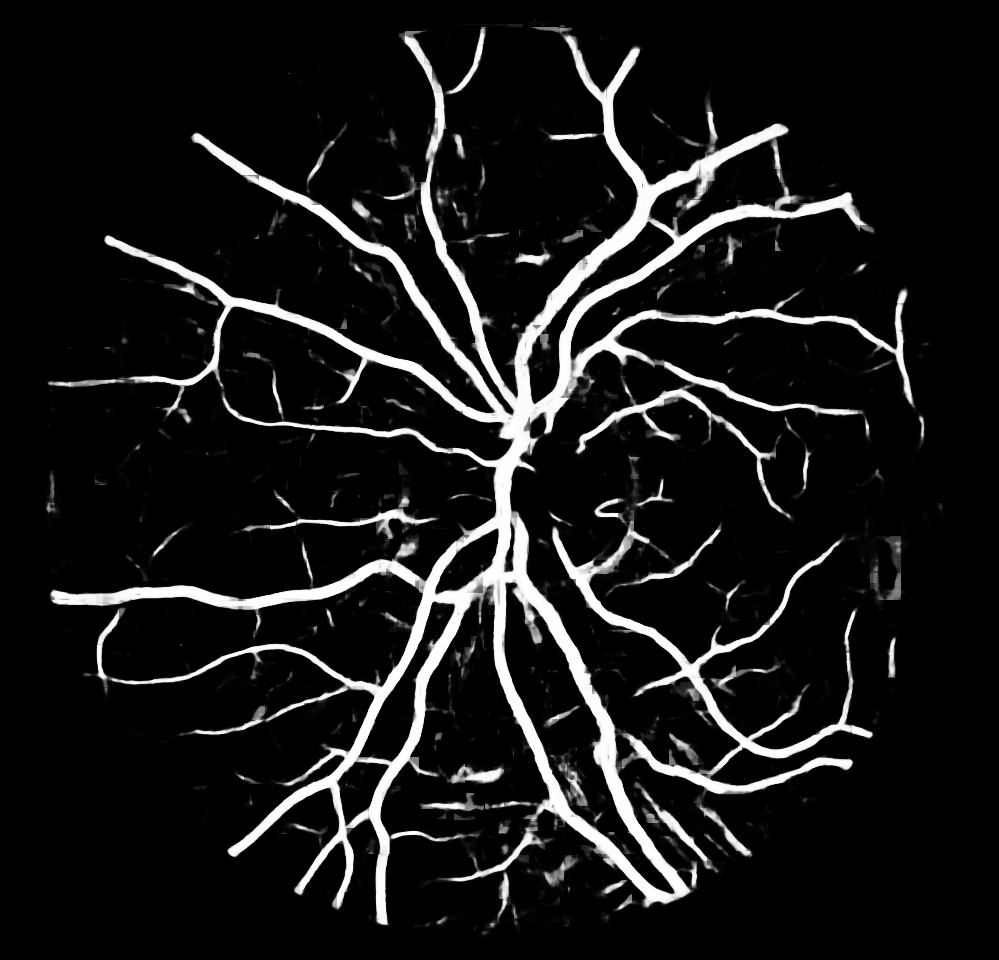
\includegraphics[width=3.6cm]{../idx1_s64_out1_p}}}\\

		\bmvaHangBox{\fbox{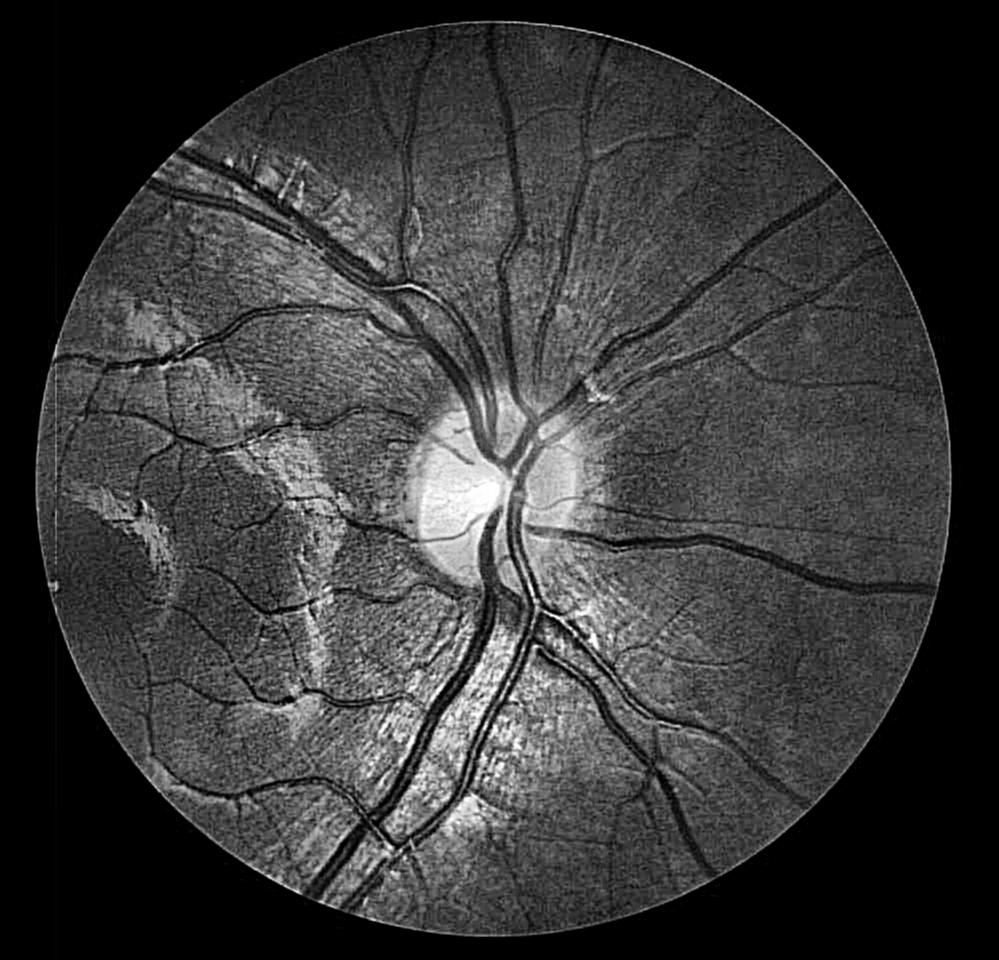
\includegraphics[width=3.6cm]{../idx2_s64_out3_x}}} &
		\bmvaHangBox{\fbox{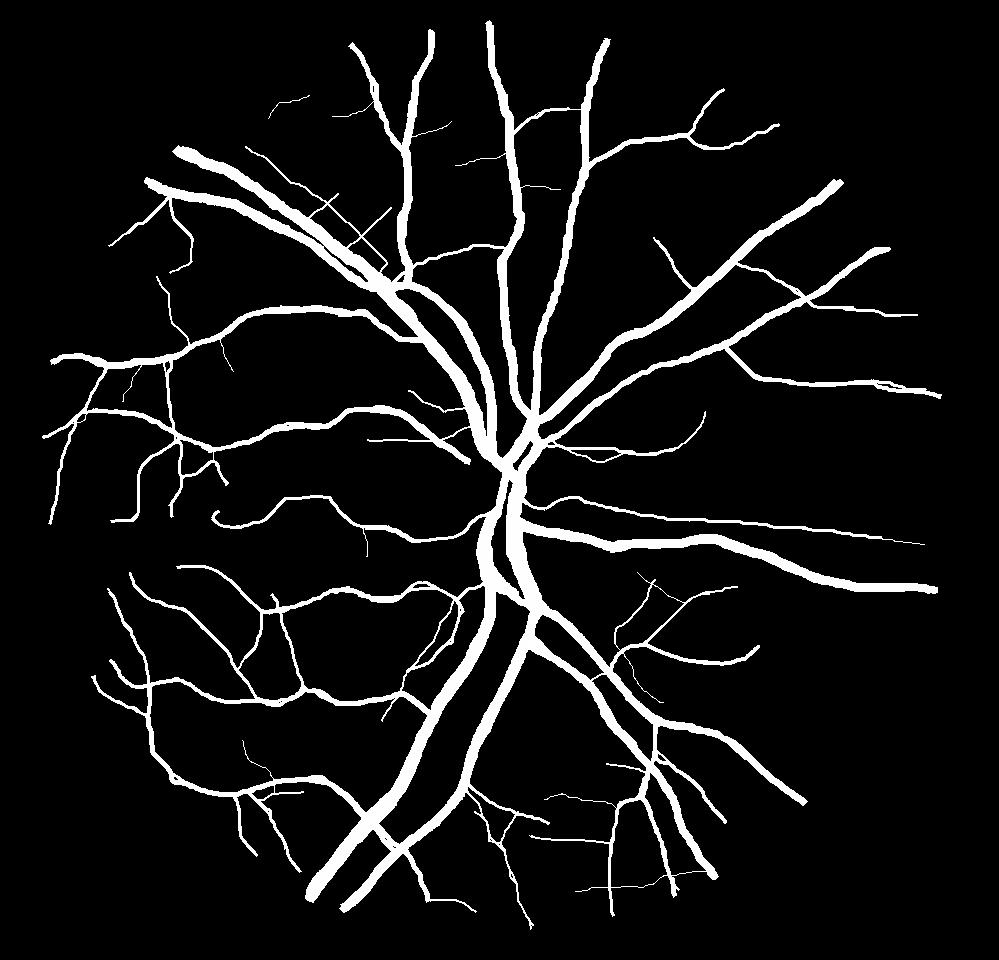
\includegraphics[width=3.6cm]{../idx2_s64_out2_y}}} &
		\bmvaHangBox{\fbox{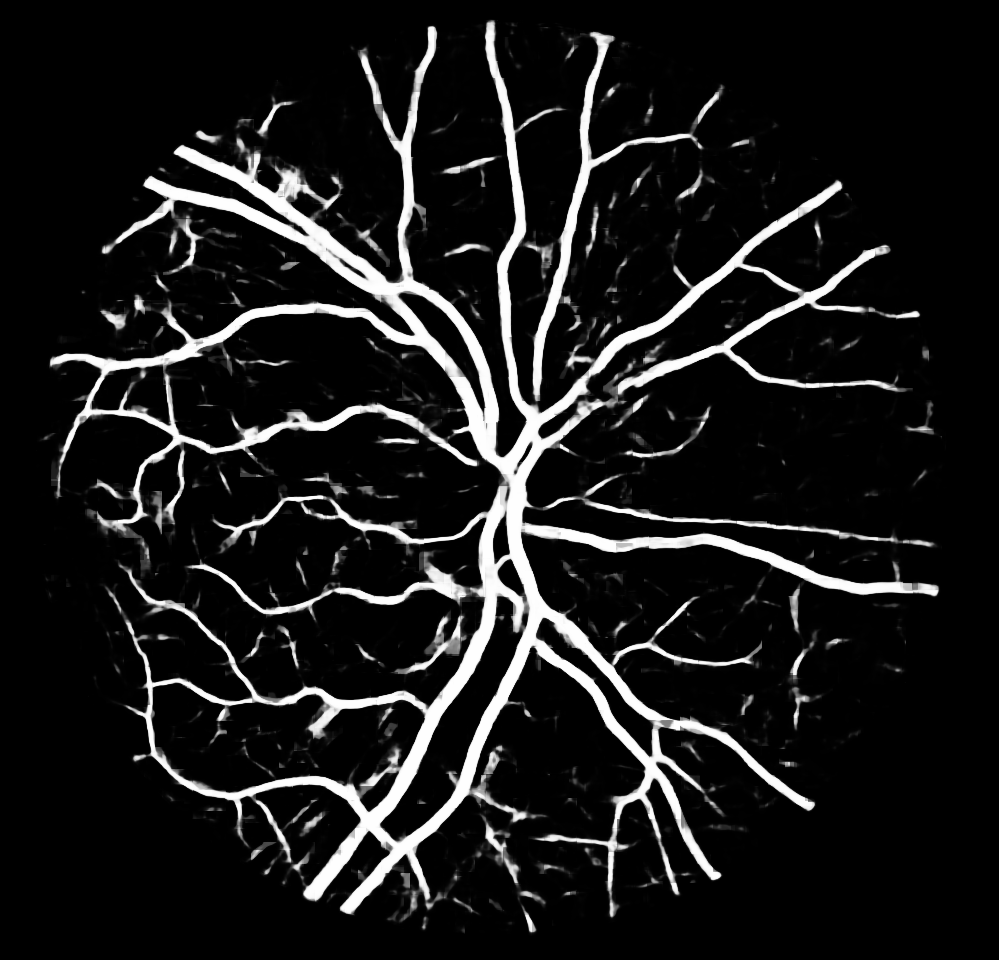
\includegraphics[width=3.6cm]{../idx2_s64_out1_p}}}\\

		\bmvaHangBox{\fbox{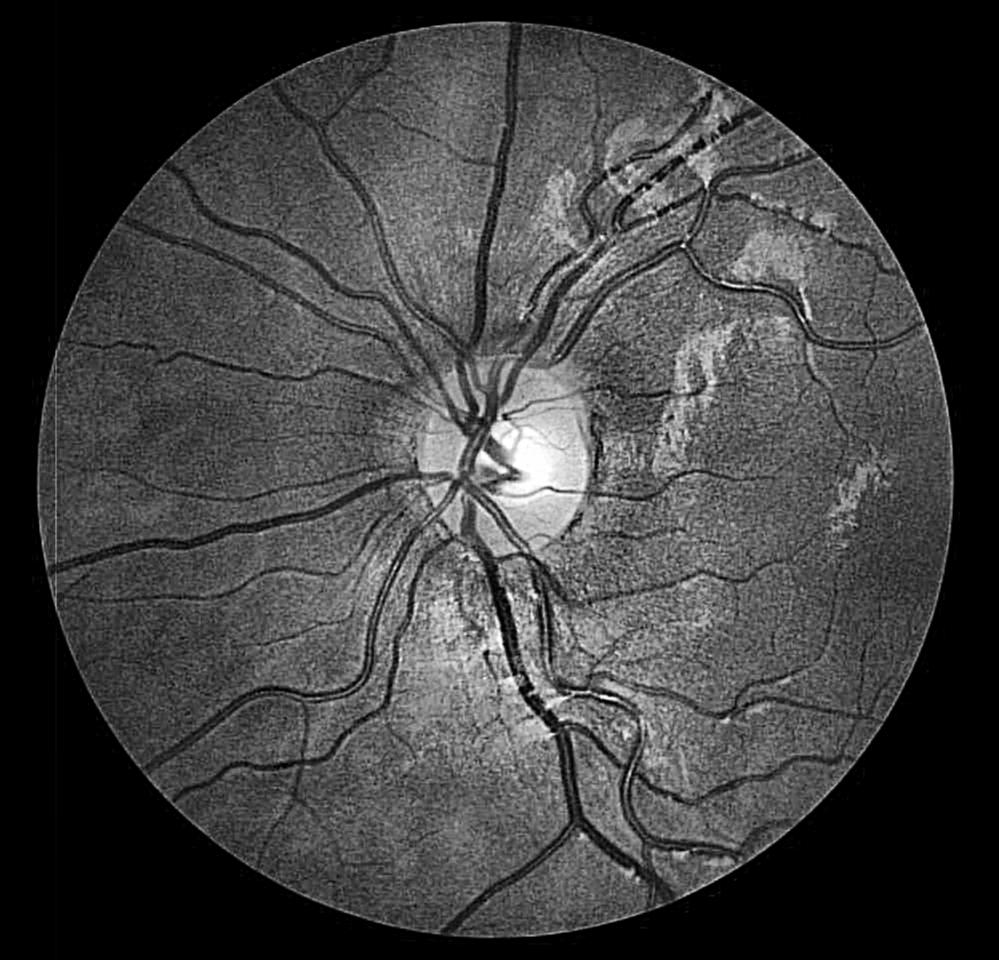
\includegraphics[width=3.6cm]{../idx3_s64_out3_x}}} &
		\bmvaHangBox{\fbox{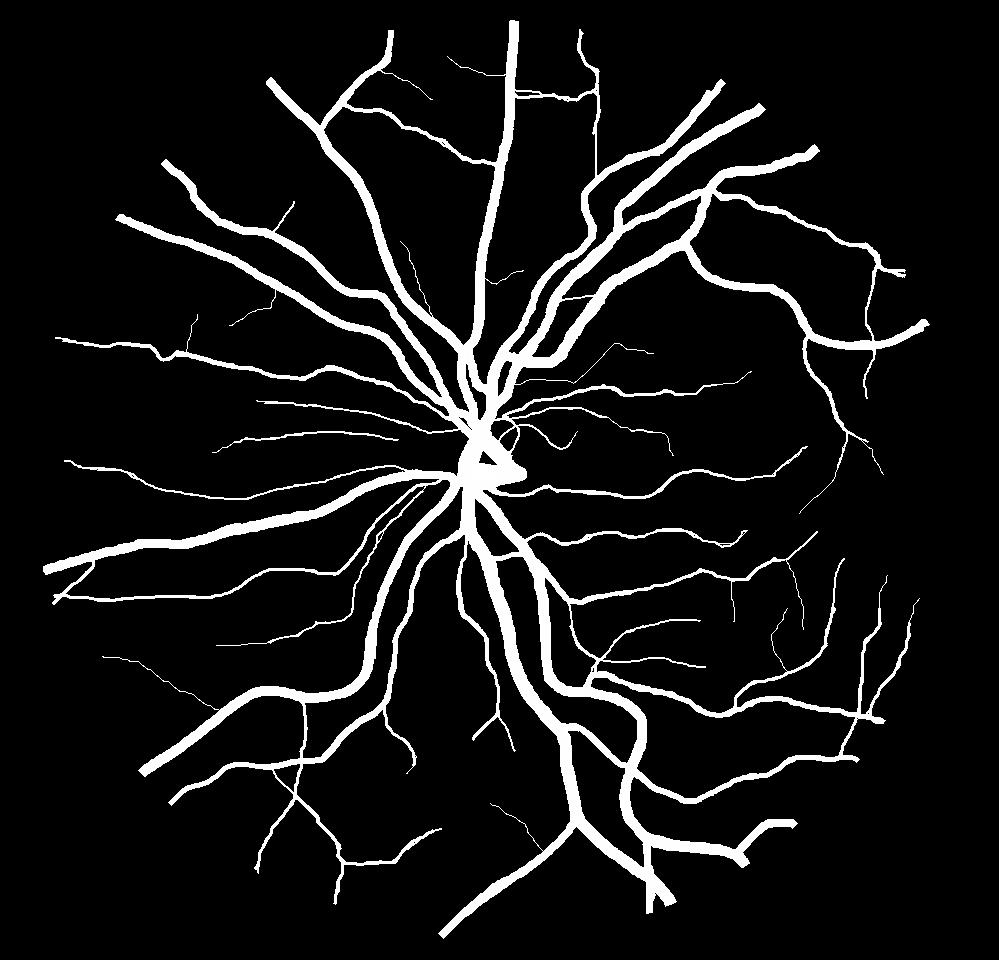
\includegraphics[width=3.6cm]{../idx3_s64_out2_y}}} &
		\bmvaHangBox{\fbox{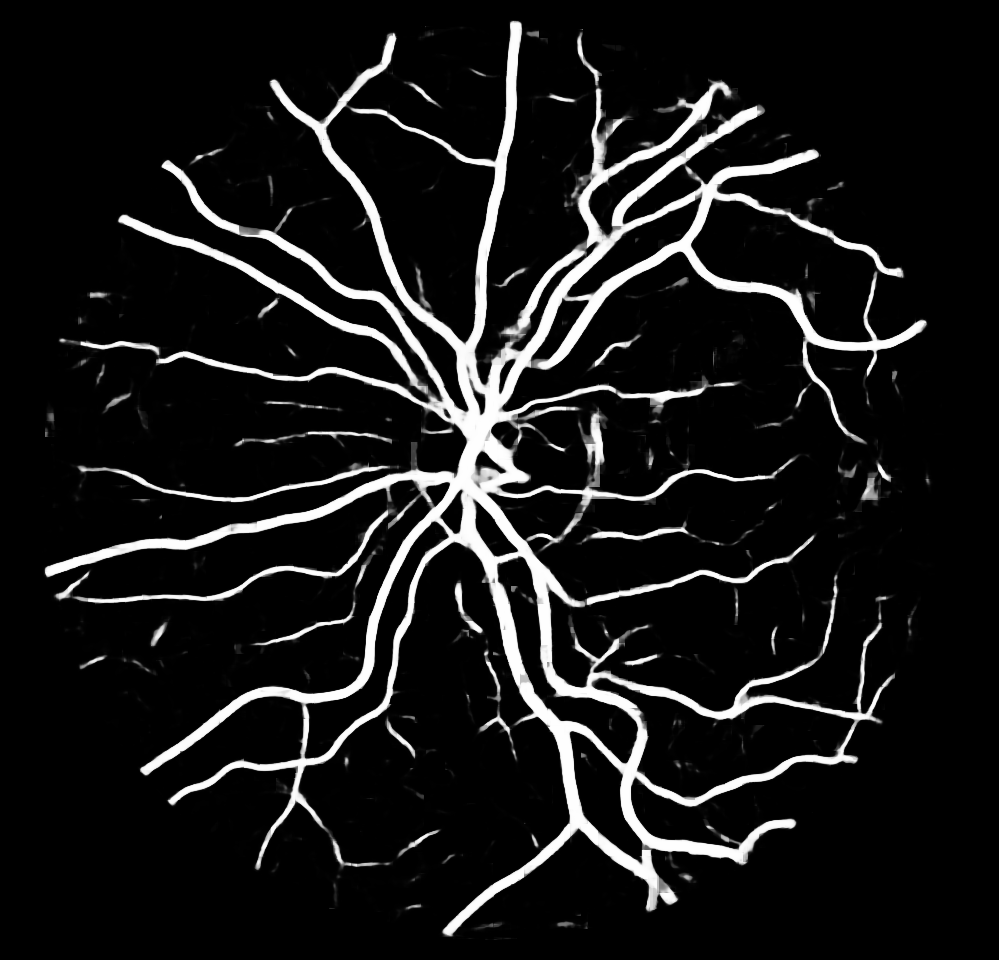
\includegraphics[width=3.6cm]{../idx3_s64_out1_p}}}\\

		\bmvaHangBox{\fbox{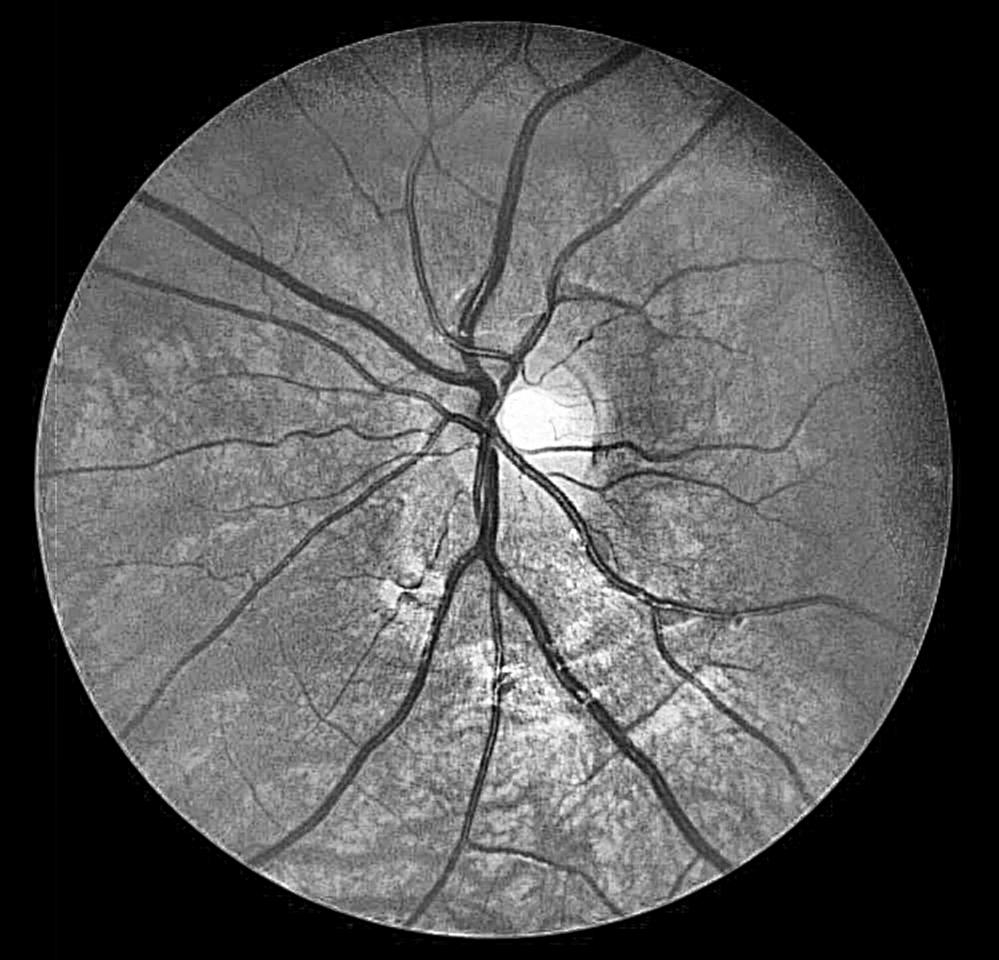
\includegraphics[width=3.6cm]{../idx4_s64_out3_x}}} &
		\bmvaHangBox{\fbox{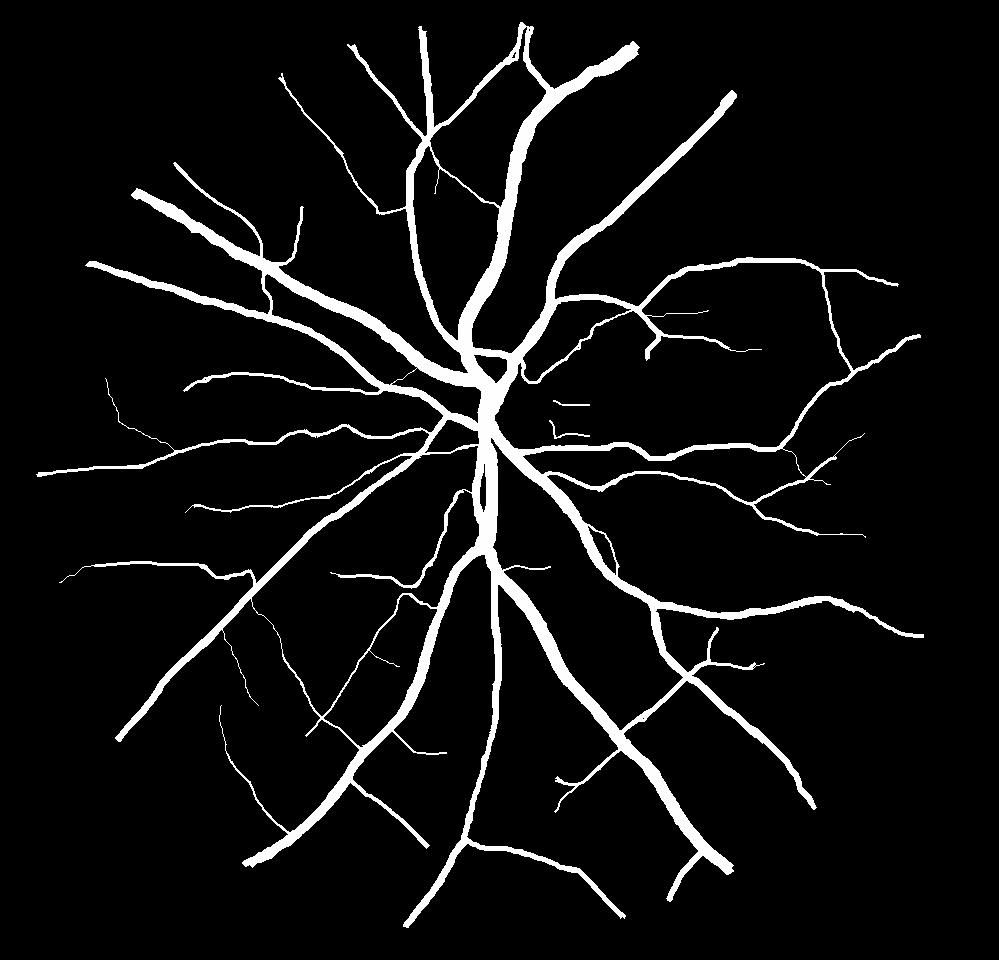
\includegraphics[width=3.6cm]{../idx4_s64_out2_y}}} &
		\bmvaHangBox{\fbox{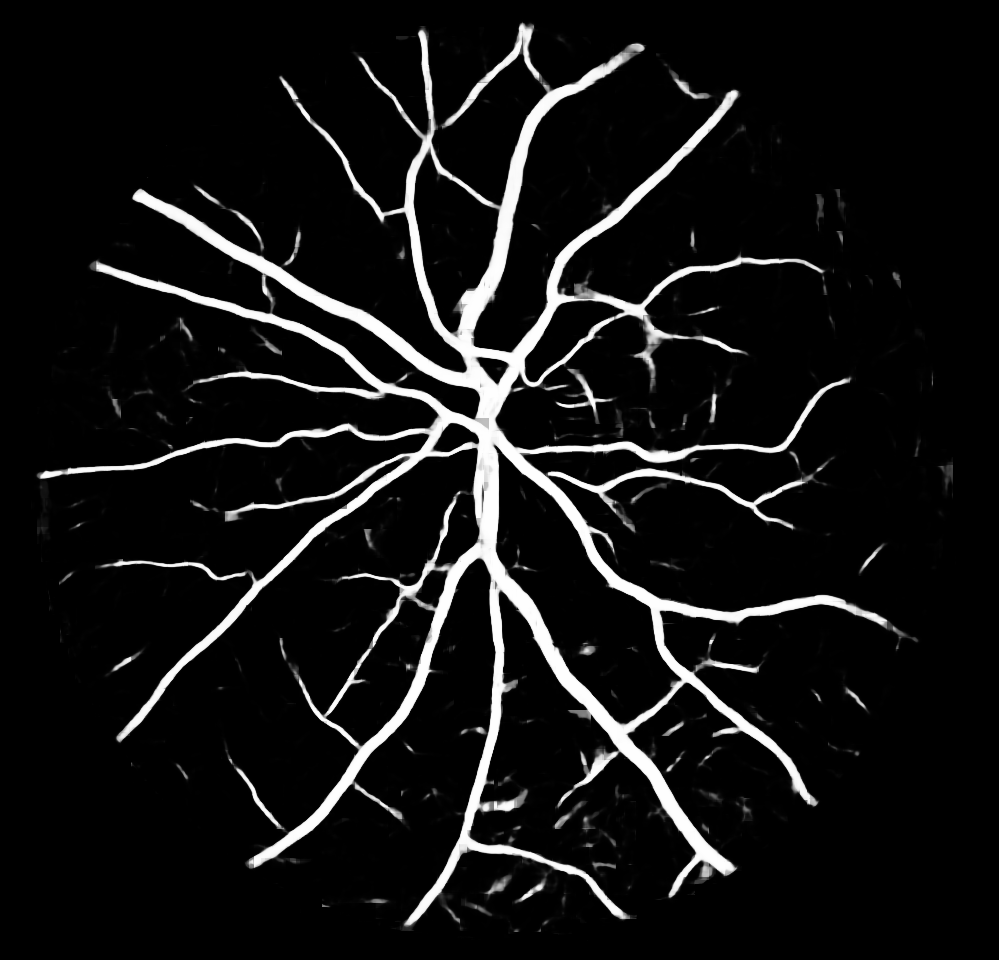
\includegraphics[width=3.6cm]{../idx4_s64_out1_p}}}\\

		(input)&(gt)&(pred)
\end{tabular}
\caption{Dla detektora 64x64px.}
\end{figure}


\section{Analiza wyników działania}

Trzeba tu podkreslic ze detektory byly trenowane mala ilosc epochow a jednak daja
calkiem przyzwoite wyniki. Najlepiej dziala dla wersji 64x64px. Przy dobrej
augumentacji oraz sprzecie byloby mozliwe wytrenowanie maski 128x128px ktora
zapewnie bylaby dobrym komprosimem pomiedzy jakoscia a szybkoscia.
Aby poprawic rezultaty moznaby po wygenerowaniu maski, potraktowac ja jeszcze
raz jakims innym modelem ktory przyjmowalby 3 wejscia: input, nasza
predykcja, wspolrzedne kwadratu wzgledem srodka oka. Taki system zapewne by
potrafil usunac szumy wokol naczyn. Aktualanej wersji usuwane sa szumu gdy
nalozy sie threshold-a 170 (dla obrazka 0 .. 255). Jednak wtedy przerywa
niektore naczynia. Wiec postanowilem zostawic orginalne wyjscia detektorow.
Analiza pojedynczych zdjec jest ujeta tabelka w poprzedniej sekcji (z {\tt
	dice\_loss}). Prosze zwrocic uwage ze kazdy przyklad w miejscu nadmiernej
ekzpozycji swiatla ma lekkie przebicie - pojawiaja sie szumy w postaci drobnych
plamek/kreseczek (mozna probowac je usunac jakims filtrem, jednak nie
przeszkadza to w intrepretacji obrazu).

\section{Uwage}

Aby przetestowac skrypt wystarczy skopiowac go do Google Colab. Instaluje on sam
potrzebne pakiety oraz sciaga moje wagi, ktore uzylem w
eksperymencie. W innym przypadku wymagany jest ponowny trening.

\end{document}
